\documentclass[11pt,aspectratio=169]{beamer}

% -------------------- THEME & LAYOUT --------------------
\usetheme{Madrid}
\usecolortheme{dolphin} % base color scheme
\usefonttheme{professionalfonts}
\setbeamercovered{transparent}
\setbeamertemplate{navigation symbols}{}   % remove navigation buttons
\setbeamertemplate{caption}[numbered]      % numbered captions
\setbeamertemplate{itemize items}[triangle]
\setbeamersize{text margin left=1.2cm,text margin right=1.2cm} % adjust to taste
% -------------------- GLOBAL FONT SETTINGS --------------------

% 1. Force the base beamer font to small
\setbeamerfont{normal text}{size=\small}

% 2. Force math environments to follow the "small" font size
\setbeamerfont{math text}{size=\small}
\setbeamerfont{equation}{size=\small}

% 3. Redefine \normalsize itself 
% This ensures equations and lists (which look for \normalsize) use  instead.
\let\oldnormalsize\normalsize
\renewcommand{\normalsize}{\oldnormalsize\small}

% 4. Ensure lists also stay small
\setbeamerfont{itemize/enumerate body}{size=\small}
\setbeamerfont{itemize/enumerate subbody}{size=\small}
% -------------------- FONTS & TYPOGRAPHY --------------------
\usepackage[T1]{fontenc}
\usepackage[utf8]{inputenc}
\usepackage{newpxtext,newpxmath} % Palatino-like font & math
\usepackage{microtype}

% -------------------- MATH, TABLES & GRAPHICS --------------------
\usepackage{amsmath,amssymb,amsfonts,mathtools}
\usepackage{bm,booktabs,siunitx,graphicx}
\graphicspath{{./}{./figures/}}
\renewcommand{\theequation}{9.\arabic{equation}}

% -------------------- UTILITIES --------------------
\usepackage{appendixnumberbeamer}
\usepackage{ragged2e}
\usepackage{xspace}
\usepackage{csquotes}
% -------------------- Bibliography --------------------
\usepackage[backend=biber,style=authoryear]{biblatex}
\addbibresource{sources.bib}
\usepackage{xcolor}

% -------------------- HYPERREF --------------------
\hypersetup{
  colorlinks=false,
  pdfauthor={Francesca},
  pdftitle={Chapter 1 — The Value of Currency}
}

% -------------------- COLORS & EMPHASIS --------------------
\definecolor{myblue}{RGB}{0,70,140}
\definecolor{myred}{RGB}{180,30,30}
\definecolor{mygreen}{RGB}{0,120,70}
\definecolor{gold}{RGB}{184,134,11}

\setbeamercolor{title}{fg=gold}       % title page
\setbeamercolor{frametitle}{fg=gold}  % slide titles
\setbeamercolor{structure}{fg=gold}   % bullets, sections, links
\setbeamercolor{section in head/foot}{fg=gold,bg=black!10} % gold text on light background

% -------------------- FOOTLINE --------------------
\setbeamertemplate{footline}{
  \leavevmode%
  \hbox{%
    % Section links (hidden if no current section)
    \begin{beamercolorbox}[wd=0.7\paperwidth,ht=2.5ex,dp=1.5ex,leftskip=1.4em]{section in head/foot}%
      \ifx\insertsection\empty
        % nothing
      \else
        Section: \insertsection
      \fi
    \end{beamercolorbox}%
    % Frame number right
    \begin{beamercolorbox}[wd=0.3\paperwidth,ht=2.5ex,dp=1.5ex,leftskip=3.8cm]{section in head/foot}%
      \insertframenumber/\inserttotalframenumber
    \end{beamercolorbox}%
  }%
  \vskip1pt%
}



\newcommand{\highlight}[1]{\textcolor{myblue}{#1}}
\newcommand{\warning}[1]{\textcolor{myred}{#1}}

% -------------------- SHORTCUTS --------------------
\newcommand{\E}{\mathbb{E}}
\newcommand{\R}{\mathbb{R}}
\newcommand{\dd}{\mathrm{d}}
\newcommand{\mc}[1]{\mathcal{#1}}
\newcommand{\bb}[1]{\mathbb{#1}}
\newcommand{\uc}{U_c}
\newcommand{\zg}{Z_g}

% -------------------- TIGHTER DISPLAY MATH --------------------
\makeatletter
\g@addto@macro\normalsize{%
  \setlength\abovedisplayskip{8pt}%
  \setlength\belowdisplayskip{8pt}%
  \setlength\abovedisplayshortskip{6pt}%
  \setlength\belowdisplayshortskip{6pt}%
}
\makeatother
\setbeamertemplate{frametitle}{
  \nointerlineskip
  \begin{beamercolorbox}[wd=\paperwidth,ht=3.5ex,dp=1ex,center]{frametitle}
    \centering\insertframetitle
  \end{beamercolorbox}
}

% -------------------- METADATA --------------------
\title[Part I — Currency and Money]{\textbf{Part I: Currency and Money}\\[2pt]\large Chapter 1 — The Value of Currency}
\subtitle{Currency, Money, and Price-Level Determination}
\author{Francesca}
\institute{}
\date{\today}

% -------------------- SECTION ROADMAP --------------------
\AtBeginSection[]
{
  \begin{frame}
    \tableofcontents[currentsection, hideothersubsections]
  \end{frame}
}


\begin{document}
\setcounter{equation}{0}


% ===================== TITLE SLIDE =====================
\begin{frame}[plain] % 'plain' removes header/footer for the title slide

\begin{columns}[T,totalwidth=\textwidth]

% ----- Left column: Main title, professor, chapter -----
\begin{column}{0.45\textwidth}
\vspace{2cm}

% Main title
{\usebeamercolor[fg]{title}\LARGE\textbf{Monetary Economics}\\[0.3cm]
\LARGE\textbf{and Policy}} 

\vspace{0.5cm}

% Professor name and date
{\large\textit{Pierpaolo Benigno}}\\[0.1cm]

\vspace{1cm}

% Chapter and subtitle
{\usebeamercolor[fg]{frametitle}\large Chapter 9: Liquidity Trap}

\end{column}

% ----- Right column: Image -----
\begin{column}{0.55\textwidth}
\vspace{1cm}
\centering
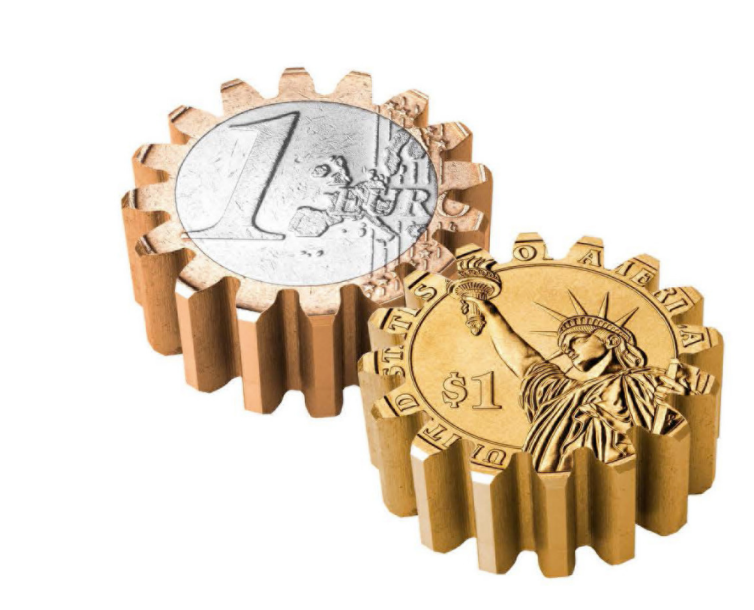
\includegraphics[width=0.9\linewidth]{Cover.png}
\end{column}

\end{columns}

% ----- Footer text (bottom-right corner) -----
\vspace*{2cm} % adjust if needed
\hfill{\large\textit{Prepared by Marcos Consuegra}}

\end{frame}
% --- NEW SLIDE: What We Will Learn ---
\begin{frame}{What We Will Learn}
\small
\begin{itemize}
  \item How a negative demand shock coupled with the \textbf{Zero Lower Bound (ZLB)} creates a liquidity trap and a shortage of aggregate demand.
  \item How \textbf{Helicopter Money} and unconventional asset-purchase programs (\textbf{QE}) can reflate the price level and stimulate consumption through explicit or implicit wealth transfers.
  \item Why pure asset swaps are neutral unless accompanied by an appropriate remittance policy that alters private-sector net worth.
  \item The role of \textbf{Forward Guidance} and price-level targeting in overcoming the ZLB, and how history dependence affects the optimal path of inflation and output.
  \item How to manage central bank  \textbf{reserves} in a liquidity trap, when taxes are distortionary, and how the central bank  acts as a \textbf{Buyer of Last Resort} to ensure financial stability.
\end{itemize}
\end{frame}
% OUTLINE
\begin{frame}{Outline}
\tableofcontents
\end{frame}

% --- SLIDE: Introduction ---
\section{Introduction}
\begin{frame}{Introduction}
\small

\begin{itemize}
    \item \textbf{Liquidity traps} describe a situation in which an economy remains in a slump due to a shortage of aggregate demand, even when the nominal interest rate is zero.
    
    \item \textbf{\cite{hicks1937}: The \enquote{Economics of Depression}}
    \begin{itemize}
        \item Describes a scenario where the $LM$ curve becomes horizontal.
        \item Any liquidity the authorities inject is absorbed without affecting either the interest rate or income.
    \end{itemize}

    \vspace{0.2cm}
    \item \textbf{The modern perspective}
    \begin{itemize}
        \item In modern central banking, the money supply is \textbf{endogenous} given the policy rate.
        \item Nevertheless, a zero floor on the interest rate exists because money can circulate in \textbf{physical form}.
        \item At the zero lower bound (ZLB), the central bank loses its standard policy instrument and must resort to unconventional measures.
    \end{itemize}
\end{itemize}

\end{frame}

\begin{frame}{Evolution of Policy Rates}
\small
{
\setbeamertemplate{caption}{\raggedright\insertcaption\par}
\begin{figure}[t]
\centering
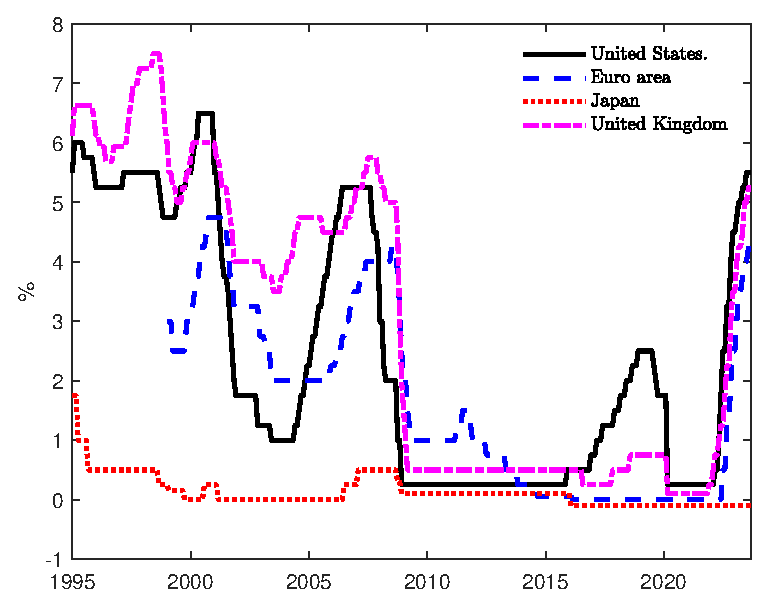
\includegraphics[width=0.55\linewidth]{Figures/Figure14.eps}
\caption{\tiny Policy rates for the Euro Area, Japan, U.K., and U.S. (Jan 1995 – Oct 2023). Source: Thomson Reuters Datastream.}
\end{figure}
}
\end{frame}

\begin{frame}{The Global Experience with the Zero Lower Bound}
\small

\begin{itemize}
  \item The \textbf{policy rate has hit the ZLB} in several advanced economies.
    \item Japan entered a period of stagnation following the collapse of the asset price bubble in 1991.
    \item Policy rates have remained below 1\% between 1995 and 2024, reaching even negative territory ($-10$ bps).
\end{itemize}

\vspace{0.2cm}

\textbf{The Global Financial Crisis and Beyond}
\begin{itemize}
    \item United States entered the ZLB in December 2008, maintaining quasi-zero rates for seven years.
    \item Euro Area shifted toward the ZLB significantly in 2014 following the sovereign debt crisis.
    \item Major central banks began a sharp \textbf{liftoff} in 2022 to combat the global surge in inflation, including Japan since 2024.
\end{itemize}

\end{frame}

\begin{frame}{Analytical Framework: The Euler Equation}
\small

\begin{itemize}
    \item To see how a demand shock and the ZLB create a shortage of aggregate demand, we consider the $AD$ equation in its non-linear Euler-equation version (5.10) under perfect foresight:
\end{itemize}
\vspace{0.3cm}
\textbf{Euler Equation}

\begin{equation}
U_{c}(C_{t})=\beta (1+i_{t}) \frac{P_{t}}{P_{t+1}} \frac{\xi_{t+1}}{\xi_{t}} U_{c}(C_{t+1})
\label{EulerLiquidity}
\end{equation}

\textbf{Interpretation}
\begin{itemize}
    \item $C_t, i_t, P_t$: Consumption, nominal interest rate, and price level.
    \item $\beta \in (0,1), \xi_t$: Subjective discount factor, preference shock.
    \item $U_c(\cdot)$: Marginal utility.
\end{itemize}

\end{frame}
% ===================== SECTION: SHORT RUN VS LONG RUN =====================
\begin{frame}{Short Run and Long Run Assumptions}
\small
\textbf{Time Horizon}
\begin{itemize}
    \item Let $t_0$ denote the \textbf{short run} and $t_0+1$ the \textbf{long run}, characterized by two fundamental assumptions:
\end{itemize}

\vspace{0.2cm}
\textbf{1. Nominal Rigidities}
\begin{itemize}
    \item \textbf{Short Run ($t_0$)}: Prices are fully rigid at $P_{t_0} = \bar{P}$.
    \item \textbf{Long Run ($t_0+1$)}: Prices are flexible at $P_{t_0+1} = P^*$, determined endogenously by monetary and fiscal policy.
\end{itemize}

\vspace{0.2cm}
\textbf{2. Preference Shock}
\begin{itemize}
    \item The preference shock is low in the short run $\xi_{t_0}$ and high in the long run $\xi_{t_0+1} = \bar{\xi}$, such that $\xi_{t_0} < \bar{\xi}$.
    \item Since $\xi$ is a multiplicative shock to the utility flow, a higher $\bar{\xi}$ implies more patient agents, creating an incentive to increase savings.
\end{itemize}
\end{frame}

\begin{frame}{Goods Market Clearing}
\small
\textbf{Goods Market Clearing}
\begin{itemize}
    \item In the long run ($t_0+1$), the absence of nominal rigidities ensures that the goods market clears.
    \vspace{0.3em}
    \item Consumption is determined by the \textbf{natural rate of output} ($Y^n$).
    \vspace{0.3em}
    \item For analytical convenience, we assume the long run natural rate of output to be constant, i.e. $Y_{t+1}^{n} = Y$, implying:
\end{itemize}
\begin{equation*}
    C_{t_{0}+1} = Y
    \label{LongRunCons}
\end{equation*}
\end{frame}

\begin{frame}{Short-Run Aggregate Demand}
\small
\begin{itemize}
    \item Substituting the information above into the Euler Equation \eqref{EulerLiquidity}, we obtain:
\end{itemize}

\begin{equation}
U_{c}(C_{t_{0}}) = \beta (1+i_{t_{0}}) \frac{\bar{P}}{P^{\ast}} \frac{\bar{\xi}}{\xi_{t_{0}}} U_{c}(Y)
\label{Liquidity}
\end{equation}

\textbf{Interpretation}
\begin{itemize}
    \item Since $U_c(\cdot)$ is a decreasing function of its argument, $C_{t_0}$ depends \textbf{negatively} on the nominal rate $i_{t_0}$.
    \item The term $\frac{\bar{\xi}}{\xi_{t_0}} > 1$ represents a \textbf{negative demand shock}. It puts upward pressure on $U_c(C_{t_0})$, which forces current consumption $C_{t_0}$ to fall.
    \item To maintain $C_{t_0} = Y$ in the face of a patience shock ($\xi_{t_0} \downarrow$), the central bank  must lower the nominal interest rate $i_{t_0}$ to offset the pressure for increased saving.
\end{itemize}
\end{frame}
\begin{frame}{Log-linear Version}
\small

\textbf{Isoelastic Utility Assumption}
\begin{itemize}
    \item Assuming $U(C) = \frac{C^{1-\sigma^{-1}}}{1-\sigma^{-1}}$, with $\sigma >0$, log-linearization of equation \eqref{Liquidity} yields:

\begin{equation}
c_{t_{0}} = y - \sigma \left(i_{t_{0}} - (p^{\ast} - \bar{p}) - r_{t_{0}}^{e} \right),
\label{Wicksell2}
\end{equation}
where the frictionless rate $r_{t_{0}}^{e}$ is defined by preference shocks:
\end{itemize}

\begin{equation*}
r_{t_{0}}^{e} = -\ln \beta + \ln \xi_{t_{0}} - \ln \bar{\xi}.
\end{equation*}
\vspace{0.2cm}
\begin{itemize}
    \item A low realization of $\xi_{t_{0}}$ (increased patience) implies a fall in $r_{t_{0}}^{e}$.
    \item \textbf{Notation}: Lowercase letters are logs and $i_{t_0} \approx \ln(1+i_{t_0})$.
\end{itemize}

\end{frame}
\begin{frame}{The Liquidity Trap Condition}
\small

\begin{itemize}
    \item If the negative shock to preferences is large enough to drive the frictionless real rate to a large negative value such that:
\begin{equation}
r_{t_{0}}^{e} + (p^{\ast} - \bar{p}) < 0,
\label{Restriction}
\end{equation}
the economy suffers a persistent shortage of aggregate demand, ($c_{t_0} < y$) , even at the zero floor ($i_{t_0} = 0$), as implied by \eqref{Wicksell2}.
\end{itemize}

\begin{itemize}
    \item \textbf{Result}: The economy finds itself in a \textbf{liquidity trap}.
\end{itemize}

\end{frame}

% --- SLIDE 1: Baseline Equilibrium ---
\begin{frame}{Graphical Analysis: Preference Shock}
\small
\begin{columns}[c]

\begin{column}{0.50\textwidth}
\textbf{The Initial State $E$}
\begin{itemize}
    \item \textbf{Supply Side}: The $AS$ curve is vertical at constant output $y$.
    \item \textbf{Demand Side}: The initial $AD$ crosses $AS$ at price $\bar{p}$ and consumption $y$. 
    \item \textbf{Policy}: The nominal rate is positive ($i_{t_0} > 0$) and the long-run price anchor is met ($\bar{p} = p^*$).
    \item \textbf{The ZLB Schedule}: $AD_0$ displays AD when $i_{t_0} = 0$.
\end{itemize}
\end{column}

\begin{column}{0.55\textwidth}
\centering
\begin{figure}
    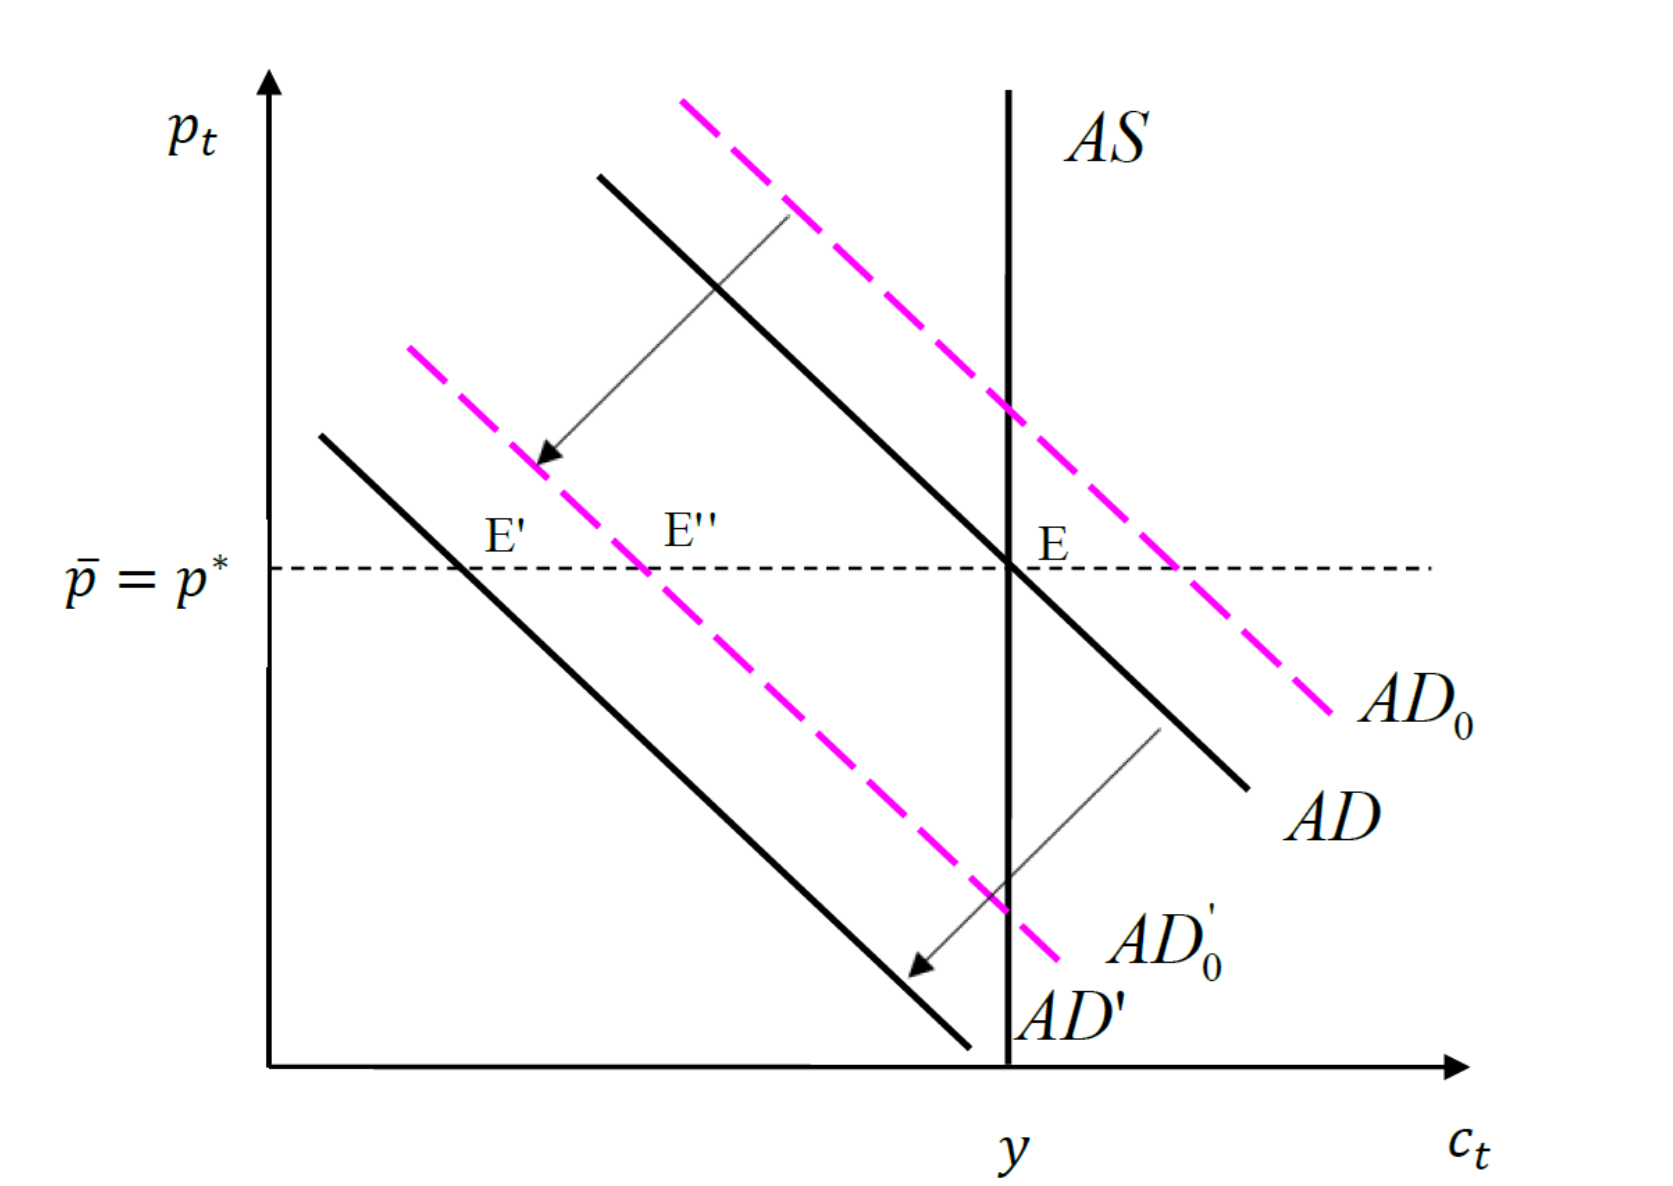
\includegraphics[width=\linewidth]{Figures/Figure15}
\end{figure}
\end{column}

\end{columns}
\end{frame}

% --- SLIDE 2: Dynamics of the Slump ---
\begin{frame}{Graphical Analysis: Dynamics of the Slump}
\small

\textbf{Preference Shock and Initial Contraction ($E \to E'$)}
\begin{itemize}
    \item A preference shock ($\xi_{t_0} \downarrow$) increases the marginal utility of future consumption, raising the desire to save.
    \item This shifts the aggregate demand schedules left.
    \item Due to short-run price rigidity at $\bar{p}$, the economy moves to equilibrium $E'$, where consumption falls strictly below potential ($c_{t_0} < y$).
\end{itemize}

\vspace{0.4cm}

\textbf{Monetary Policy Response and the Trap ($E' \to E''$)}
\begin{itemize}
    \item The central bank  can attempt to offset the demand deficiency by lowering $i_{t_0}$, shifting $AD'$ at most to $AD'_0$.
    \item \textbf{The Liquidity Trap}: The new equilibrium is $E''$. Despite $i_{t_0} = 0$, the real interest rate remains too high to clear the goods market, leaving the economy in a persistent slump.
\end{itemize}

\end{frame}

% --- SLIDE 3: Necessary Conditions ---
\begin{frame}{Prerequisites for a Liquidity Trap}
\small

\textbf{Three Necessary Conditions}
\begin{itemize}
    \item \textbf{Negative Demand Shock}: Preference shifts ($\xi \downarrow$) that push $r^e$ into negative territory.
    \item \textbf{Price Rigidities}: Prevents the price level from falling to clear the goods market.
    \item \textbf{Zero Lower Bound (ZLB)}: A floor on nominal rates due to the existence of physical currency.
\end{itemize}

\vspace{0.4cm}

\textbf{No Liquidity Trap occurs under:}
\begin{itemize}
    \item \textbf{Flexible Prices}: The goods market clears even in the short run via price adjustment.
    \item \textbf{No ZLB Constraint}: The central bank  sets $i_{t_0} < 0$ to bridge the demand gap.
\end{itemize}

\end{frame}

% --- SLIDE 4: The Real Rate and Inflation Expectations ---
\begin{frame}{Note: The Real Rate and Inflation Expectations}
\small
\textbf{The Real Rate Disconnect}
\begin{itemize}
    \item Real rate definition: $r_{t_{0}} = i_{t_{0}} - (p^{\ast} - \bar{p})$.
    \item A liquidity trap arises when the actual real rate is \enquote{too high} relative to the frictionless rate: $r_{t_0} > r_{t_0}^e$.
    \item This disconnect creates \textbf{excess saving}, depressing current consumption and aggregate demand.
\end{itemize}

\vspace{0.4cm}
\textbf{Exiting the Trap: The Role of Inflation Expectations}
\begin{itemize}
    \item Since $i_{t_0}$ is constrained by the ZLB, the real rate can also fall to align with the frictionless rate through a rise in \textbf{inflation expectations}, i.e. $p^{\ast}$ goes up.
\end{itemize}
\end{frame}

% -------------------- Outline of the Results --------------------
\section{Outline of the Results}
\begin{frame}{Outline of the Results}
\small

This chapter studies tools to escape the liquidity trap when conventional monetary policy is constrained. The main results are:

\begin{itemize}
    \item \textbf{Helicopter Money}: Direct transfers to the private sector stimulate aggregate demand through a \textbf{wealth effect}, effectively increasing consumption and inflation.
    \item \textbf{Asset Purchase Programs}: By absorbing private sector risk, these programs generate \textbf{implicit transfers} that bolster net worth and elevate inflation expectations.
    \item \textbf{Forward Guidance}: Managing future policy rate trajectories to boost inflation expectations and reduce current/future real rates.
    \item \textbf{Reserve Management}: The optimal accumulation and withdrawal of central bank  reserves to manage liquidity when taxation is distortionary.
    \item \textbf{Lender of Last Resort}: Mitigating systemic risk by providing liquidity against illiquid assets to alleviate credit market constraints.
\end{itemize}

\end{frame}

\section{Helicopter Money}

% --- SLIDE: Helicopter Money ---
\begin{frame}{Helicopter Money: Theoretical Framework}
\small

\textbf{The \textcite{friedman1969optimum} Paradigm}
\begin{itemize}
    \item A unique, non-recurrent event where currency is dropped to the community.
    \item \textbf{Monetary Logic}: Deflation is a state where the price of currency is too high. Since central banks print default-free liabilities, they can \textbf{reflate} the economy by increasing the supply of these units as a permanent "gift".
\end{itemize}

\vspace{0.4cm}

\textbf{Transmission Mechanism}
\begin{itemize}
    \item \textbf{Reflation}: Stimulates demand by raising long-run price expectations ($p^*$), which lowers current real interest rates.
    \item \textbf{Operational Step}: The Treasury issues debt to fund private-sector transfers, which the central bank  monetizes via permanent reserve expansion.
    \item \textbf{The Wealth Effect}: Unlike standard debt-financed transfers, this injection is not offset by future tax liabilities, leading to a permanent increase in private nominal net worth.
\end{itemize}

\end{frame}
% --- SLIDE 1: Empirical Evidence of Policy Coordination ---
\begin{frame}{U.S. Federal Debt and Federal Reserve Holdings}
\small
\begin{columns}[c]

\begin{column}{0.40\textwidth}
\begin{itemize}
    \item \textbf{Coordination}: Episodes of fiscal–monetary alignment have been frequent since 2007. The surges in federal debt and Federal Reserve holdings have mirrored each other.
    \item \textbf{Monetization}: This could represent the operational outcome of a \enquote{helicopter drop}.
\end{itemize}
\end{column}

\begin{column}{0.60\textwidth}
\centering
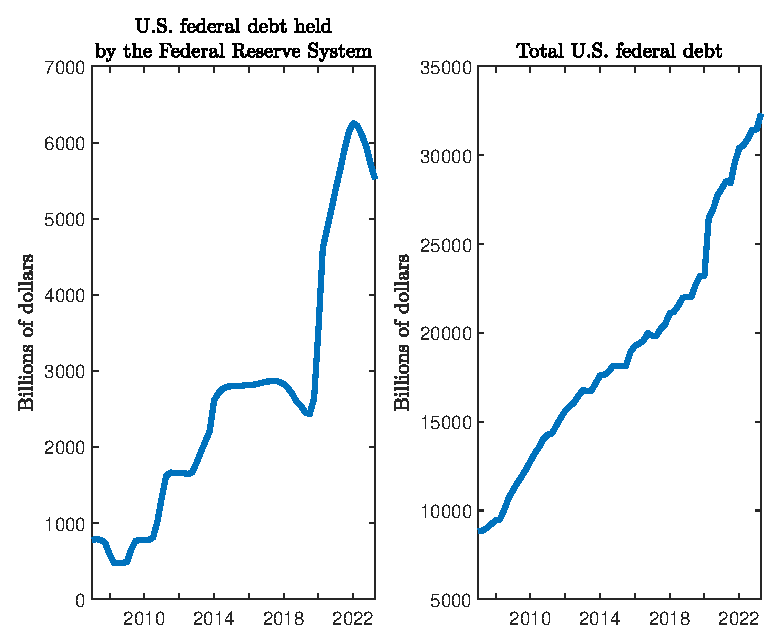
\includegraphics[width=\linewidth]{Figures/Figure16.eps}
\textit{\tiny{Source: St. Louis Fed.}}
\end{column}

\end{columns}
\end{frame}

% --- SLIDE 2: Case Study: United States Experience ---
\begin{frame}{United States: Crisis Interventions}
\small

\textbf{2007--2008 Financial Crisis}
\begin{itemize}
    \item \textbf{Fiscal}: American Recovery and Reinvestment Act (\$787bn stimulus) launched in February 2009.
    \item \textbf{Monetary}: QE1 launched (\$300bn in long-term debt and MBS) in March 2009; QE2 expanded purchases by \$600bn in November 2010.
\end{itemize}

\vspace{0.2cm}

\textbf{COVID-19 Pandemic Relief (March 2020 -- March 2021)}
\begin{itemize}
    \item \textbf{Fiscal}: Five stimulus packages totaling over \$5tn, featuring direct cash transfers, tax credits, and expanded unemployment benefits.
    \item \textbf{Monetary}: The Federal Reserve accumulated $\approx$\$3tn in Treasury securities and implemented direct/indirect lending to small and medium-sized businesses.
\end{itemize}

\end{frame}

% --- SLIDE 3: Case Study: European Experience ---
\begin{frame}{Europe: Pandemic Emergency Purchase Programme (PEPP)}
\small

\textbf{ECB Monetary Expansion \& Fiscal Coordination}
\begin{itemize}
    \item Activation of PEPP at €1.8 trillion, purchasing sovereign debt of euro-area national treasuries.
    \item \textit{Note}: Unlike the 2015 QE, this was explicitly linked to a coordinated fiscal expansion.
    \item The European Commission relaxed the 3.0\% deficit rule, allowing for substantial national deficits.
    \item Implementation of a €800 billion European-wide fiscal stimulus.
\end{itemize}

\end{frame}

\begin{frame}{Model}
\small
Consider a representative household's intertemporal utility including also real money balances (see Chapter 2):
\begin{equation*}
\sum_{t=t_{0}}^{\infty }\beta ^{t-t_{0}}\xi _{t}\left[ U(C_{t}) + V\left( \frac{M_{t}}{P_{t}} \right) \right]. 
\end{equation*}


\textbf{Interpretation}
\begin{itemize}
    \item $M_t$: Cash.
    \item $V(\cdot)$: utility in real money balances $M_t/P_t$.
    \item $V(\cdot)$ has a satiation point at $\bar{m} > 0$:
    \begin{equation*}
    V_{m}\left( \frac{M_t}{P_t} \right) = 0 \quad \text{for} \quad \frac{M_t}{P_t} \geq \bar{m}.
    \end{equation*}
\end{itemize}
\end{frame}
\begin{frame}{Structural Assumptions}
\small
\begin{itemize}
    \item \textbf{Preference Shock}: $\xi _{t}=\bar{\xi}$ for each $t\geq t_{0}+1$ while $\xi _{t_{0}}\leq \bar{\xi}$.
    \vspace{0.25em}
    \item \textbf{Short Run ($t_0$)}: Prices are fixed at $\bar{P}$.
    \vspace{0.25em}
    \item \textbf{Long Run ($t \geq t_0+1$)}: Prices are fully flexible.
    \vspace{0.25em}
    \item \textbf{Equilibrium}: Price flexibility and constant endowment imply $C_{t}=Y$ for each $t\geq t_{0}+1$.
\end{itemize}

\end{frame}

\begin{frame}{Short-Run Equilibrium Conditions}
\small

\begin{itemize}
    \item Using the above assumptions into the Euler equation (\ref{EulerLiquidity}):
\end{itemize}
\textbf{Euler Equation}
\begin{equation}
U_{c}(C_{t_{0}})=\beta (1+i_{t_{0}})\frac{\bar{P}}{P_{t_{0}+1}}\frac{\bar{\xi}}{\xi _{t_{0}}}U_{c}(Y). \label{Euler-L}
\end{equation}

\vspace{0.4cm}

\begin{itemize}
    \item As discussed in Chapter 2, equilibrium in the money market implies at time $t_0$:
\begin{equation*}
\frac{M_{t_{0}}}{\bar{P}}\geq L(C_{t_{0}},i_{t_{0}}).
\end{equation*}
    \item \textbf{At the ZLB}: When $i_{t_0} = 0$, agents are indifferent between holding money and bonds. The money supply $M_{t_0}$ is absorbed with the inequality holding strictly.
\end{itemize}

\end{frame}

\begin{frame}{Long-Run Price Determination }
\small
\begin{itemize}
    \item The price level $P_{t_0+1}$ is endogenously determined by the equilibrium conditions discussed in \textbf{Chapter 2}. We restate them:
\end{itemize}

\vspace{0.3cm}
\textbf{The Fisher Equation}
\begin{itemize}
    \item Relates the nominal rate to the real rate ($1/\beta$) and inflation:
    \begin{equation}
    1+i_{t}=\frac{1}{\beta }\frac{P_{t+1}}{P_{t}}  \label{Fisher-L}.
    \end{equation}
\end{itemize}

\vspace{0.2cm}
\textbf{Money Market Equilibrium}
\begin{itemize}
    \item Real balances satisfy the liquidity preference relationship:
    \begin{equation}
    \frac{M_{t}}{P_{t}}\geq L(Y,i_{t}), \label{Money-L}
    \end{equation}
    holding with equality whenever $i_{t}>0$, Note that consumption is equal to $Y$ in the long run.
\end{itemize}
\end{frame}

\begin{frame}{Intertemporal Budget Constraint}
\small
\begin{itemize}
    \item Following the household's optimization in \textbf{Chapter 2}, the intertemporal budget constraint must be satisfied in equilibrium:
\end{itemize}
\vspace{0.3cm}
\textbf{Intertemporal Budget Constraint}

\begin{equation}
\sum_{t=t_{0}+1}^{\infty }\beta ^{t-t_{0}-1}\left( \frac{T_{t}}{P_{t}}+\frac{i_{t}}{1+i_{t}}\frac{M_{t}}{P_{t}}\right) =\frac{B_{t_{0}}+X_{t_{0}}+M_{t_{0}}}{P_{t_{0}+1}}.  \label{IBC-L}
\end{equation}

\vspace{0.4cm}
\textbf{Interpretation}
\begin{itemize}
    \item $B_{t_0}$: Treasury bonds at time $t_0$.
    \item $X_{t_0}$: central bank  reserves at time $t_0$.
\end{itemize}
\end{frame}

% --- SLIDE: The central bank  Budget Constraint ---
\begin{frame}{Central Bank Budget Constaint}
\small

\textbf{Flow Budget Constraint}
\begin{equation}
\frac{B_{t}^{C}-X_{t}}{1+i_{t}}-M_{t}=B_{t-1}^{C}-X_{t-1}-M_{t-1}-T_{t}^{C}.
\label{BudgetC-L}
\end{equation}

\vspace{0.4cm}

\textbf{Interpretation}
\begin{itemize}
    \item $B_{t}^{C}$: Holdings of short-term, default-free assets (private or treasury).
    \item $T_{t}^{C}$: Remittances transferred to the treasury (if $T^C > 0$).
\end{itemize}
\end{frame}

% --- SLIDE: The Treasury Budget Constraint ---
\begin{frame}{Treasury Budget Constraint}
\small

\textbf{Flow Treasury Budget Constraint}
\begin{equation}
\frac{B_{t}^{F}}{1+i_{t}}=B_{t-1}^{F}-T_{t}-T_{t}^{C},\ \text{where $B_{t}^{F}$ is treasury debt.}  \label{BudgetF-L}
\end{equation}
\vspace{0.3cm}

\textbf{Solvency Constraint}
\begin{itemize}
    \item The trajectory of taxes $T$ is constrained by intertemporal solvency:
\end{itemize}
\begin{equation}
\frac{B_{t_{0}}^{F}}{P_{t_{0}+1}}=\sum_{t=t_{0}+1}^{\infty }\beta ^{t-t_{0}-1}\left( \frac{T_{t}}{P_{t}}+\frac{T_{t}^{C}}{P_{t}}\right). 
\label{Solvency-L}
\end{equation}
\textbf{Debt Market Clearing}

\begin{equation}
B_{t}^{F}=B_{t}+B_{t}^{C}.  \label{Bond-L}
\end{equation}


\end{frame}

\begin{frame}{Equilibrium Definition}
\small
\textbf{Long-run equilibrium:}  
A set of sequences
\[
\{ P_t, i_t, X_t, M_t, B_t, B_t^C, B_t^F, T_t, T_t^C \}_{t=t_0+1}^\infty,
\]
with $\{ P_t, i_t, X_t, M_t, B_t^C \}_{t=t_0+1}^\infty \ge 0$, satisfying, for all $t \ge t_0+1$:
\begin{itemize}
  \item Fisher equation \eqref{Fisher-L}
  \item Money market equilibrium \eqref{Money-L}
  \item central bank  budget constraint \eqref{BudgetC-L}
  \item Treasury budget constraint \eqref{BudgetF-L}
  \item Bond market clearing \eqref{Bond-L}
\end{itemize}
and satisfying the private sector intertemporal budget constraint \eqref{IBC-L}
given inherited values from period $t_0$:
\[
B_{t_0}^C,\; B_{t_0}^F,\; X_{t_0},\; M_{t_0}.
\]
The sequence of taxes $\{T_t\}_{t=t_0+1}^\infty$ is restricted to satisfy the
Treasury solvency condition \eqref{Solvency-L}, given equilibrium sequences
$\{P_t, T_t^C\}_{t=t_0+1}^\infty$ and the inherited value $B_{t_0}^F$.
\end{frame}
% --- SLIDE 1: Policy Regime ---
\begin{frame}{Case 1: Helicopter Money under Coordinated Policy}

\textbf{Monetary and Fiscal Policy Coordination}
\vspace{1em}
\begin{itemize}
    \item This regime relies on the \textbf{backing of Treasury liabilities by the central bank }.
\vspace{1em}
    \item The central bank's guarantee on Treasury debt relaxes the standard Treasury solvency constraint \eqref{Solvency-L}.
\end{itemize}
\end{frame}

\begin{frame}{Determination of the Price Sequence}
\small
\textbf{Interest-rate Policy Assumption}
\begin{itemize}
    \item For all $t \ge t_0+1$, the central bank  commits to a constant inflation target $\Pi > \beta$:
    \begin{equation*}
        1+i_t = \frac{\Pi}{\beta} \implies \frac{P_{t+1}}{P_t} = \Pi,
    \end{equation*}
    pinning down the path of inflation and interest rates through the Fisher equation \eqref{Fisher-L}, given $P_{t_{0}+1}$.
    
    \item Given the interest-rate policy, real money balances \eqref{Money-L} for $t \ge t_0+1$ are constant:
    \begin{equation*}
        \frac{M_t}{P_t} = L\!\left(Y,\frac{\Pi}{\beta}-1\right),
    \end{equation*}
    pinning down the path of money holdings $M_t$ for $t \ge t_0+1$, given $P_{t_{0}+1}$.
\end{itemize}
\end{frame}

% --- SLIDE 2: Money Market and Seigniorage ---
\begin{frame}{Nominal Anchor}
\small
\begin{itemize}
    \item The level of prices $P_{t_{0}+1}$ still needs to be determined.
\end{itemize}
\vspace{0.3cm}
\textbf{Real Tax Policy Assumption}
\begin{itemize}
    \item[] % Using an empty item for alignment
    \begin{equation*}
        \frac{T_t}{P_t} = (1-\beta)\tau, \quad \tau > 0.
    \end{equation*}
    \item Substituting the tax policy and seigniorage into the IBC \eqref{IBC-L}:
    \begin{equation*}
        \frac{B_{t_0}+X_{t_0}+M_{t_0}}{P_{t_0+1}} = \tau + \mathcal{S}(\Pi,Y),
    \end{equation*}
    where
    \begin{equation*}
\mathcal{S}(\Pi,Y) \equiv \sum_{t=t_{0}+1}^{\infty }\beta ^{t-t_{0}-1}\frac{i_{t}}{1+i_{t}}\frac{M_{t}}{P_{t}}  = \frac{\Pi-\beta}{\Pi(1-\beta)} L\Big(Y, \frac{\Pi}{\beta}-1\Big).
    \end{equation*}
\end{itemize}
\end{frame}

% --- SLIDE 3: Price-Level Determination ---
\begin{frame}{Price-Level Determination under Coordination}
\small

\textbf{The Nominal Anchor}
\begin{equation}
    P_{t_0+1} = \frac{B_{t_0}+X_{t_0}+M_{t_0}}{\tau + \mathcal{S}(\Pi,Y)} \label{Plong}
\end{equation}
\vspace{0.3cm}
\begin{itemize}
    \item The long run price level is proportional to the outstanding government liabilities carried from the short run (time $t_0$).
    \item Increasing them raises the price level proportionally.
\end{itemize}
\end{frame}
% --- SLIDE 4: Implementing the Helicopter Drop ---
\begin{frame}{Reflating and Stimulating Aggregate Demand}
\small
\textbf{Policy Objective to Exit the Liquidity Trap}
\begin{itemize}
    \item The government should \textbf{reflate the economy} by raising $P_{t_0+1}$ and \textbf{stimulating consumption} $C_{t_0}$ via the Euler equation \eqref{Euler-L}.
\end{itemize}

\vspace{0.3cm}

\textbf{The "Helicopter Drop" Mechanism}
\begin{itemize}
    \item A cut in taxes $T_{t_0}$ at time $t_0$ is financed by increasing nominal liabilities ($B_{t_0}, X_{t_0}, \text{ or } M_{t_0}$). 
    \item \textbf{Liability Equivalence:} Since the short-run nominal interest rate is zero ($i_{t_0}=0$), the composition of these liabilities does not matter.
\end{itemize}
\end{frame}

% --- SLIDE 5: Effects of Helicopter Money ---
\begin{frame}{The Impact on the Price Level}
\small
\begin{itemize}
    \item Consolidating the  central bank  \eqref{BudgetC-L} and Treasury \eqref{BudgetF-L} budgets at $t_0$ (with $i_{t_0}=0$):
        \vspace{0.3cm}

    \begin{equation}
        B_{t_0}+X_{t_0}+M_{t_0} = B_{t_0-1}+X_{t_0-1}+M_{t_0-1} - T_{t_0} \label{IBB2}
    \end{equation}
    \vspace{0.3cm}
        \item A lower $T_{t_0}$ (tax cut) increases total nominal liabilities in \eqref{IBB2}.

    \vspace{0.3cm}

        \item From \eqref{Plong}, if the real backing ($\tau$ and $\mathcal{S}$) remains constant, the increase in the numerator leads to a proportional increase in $P_{t_0+1}$.
\end{itemize}
\end{frame}

% --- SLIDE 6: Deficit Financing and Equivalence ---
\begin{frame}{Liability Equivalence}
\small

\textbf{Irrelevance of Asset Composition}
\begin{itemize}
    \item The $t_0$ tax cut defined in \eqref{IBB2} can be financed through two equivalent channels:
    \begin{itemize}
        \item \textbf{Private Sector:} The Treasury issues debt $B_{t_0}$ directly to the public.
        \item \textbf{Central Bank:} The Bank issues liabilities $X_{t_0}$ (reserves) to purchase Treasury debt.
    \end{itemize}
    \item At the ZLB ($i_{t_0}=0$), these financing options are perfect substitutes.
    \item Large-scale asset purchases produce equivalent effects regardless of whether the program targets short-term or long-term debt instruments.
    \item It is analytically irrelevant whether the central bank  holds the Treasury debt permanently or writes it off.
    \item The economic impact depends solely on the \textbf{unbacked} transfer made to the private sector.
\end{itemize}
\end{frame}
% --- SLIDE 7: The Mechanism of Permanent Reflation ---
\begin{frame}{Requirements and Mechanism}
\small

\textbf{Permanent Unbacked Liability Expansion}
\begin{itemize}
    \item Effectiveness depends on a constant denominator ($\tau + \mathcal{S}$) in \eqref{Plong}.
    \item Therefore, the Treasury must commit to \textbf{never undo the} tax relief.
\end{itemize}

\vspace{0.4cm}

\textbf{Transmission Channel}
\begin{itemize}
    \item \textbf{Wealth Effect:} Increased nominal liabilities (helicopter drop) raise household net wealth.
    \item \textbf{Excess Demand:} With output $Y$ fixed, stimulated consumption cannot be met by higher production.
    \item \textbf{Price Adjustment:} The resulting excess demand is fully absorbed by a proportional increase in the price level $P_{t_0+1}$.
\end{itemize}
\end{frame}

% --- SLIDE 8: Independent central bank  Regime ---
\begin{frame}{Case 2: Helicopter Money by Central Bank  Only}
\small

\textbf{Institutional Setting}
 \vspace{0.2cm}
\begin{itemize}
    \item We consider a regime where the central bank  does not back Treasury liabilities, as discussed in Chapter 1, and study whether similar Helicopter money experiments can be undertaken.
    \vspace{0.2cm}
    \item The Treasury must remain solvent independently, satisfying \eqref{Solvency-L}.
    \vspace{0.2cm}
    \item Combining the solvency constraint \eqref{Solvency-L} with the intertemporal budget constraint \eqref{IBC-L} yields:
\end{itemize}

\begin{equation}
\frac{X_{t_{0}}+M_{t_{0}}-B_{t_{0}}^{C}}{P_{t_{0}+1}}=\sum_{t=t_{0}+1}^{\infty }\beta ^{t-t_{0}-1}\left( \frac{i_{t}}{1+i_{t}}\frac{M_{t}}{P_{t}}-\frac{T_{t}^{C}}{P_{t}}\right). \label{KeyCB}
\end{equation}
\end{frame}

% --- SLIDE 9: Policy Assumptions and the Nominal Anchor ---
\begin{frame}{The Nominal Anchor}
\small

\textbf{Policy Assumptions}
 \vspace{0.2cm}
\begin{itemize}
    \item \textbf{Constant inflation target:} $\Pi > \beta$ and $1+i_t = \frac{\Pi}{\beta}$.
    \item \textbf{Constant Remittances:} Nominal policy $\{T_{t}^{C}=T^{C}\}_{t=t_{0}+1}^{+\infty }$.
\end{itemize}

\vspace{0.2cm}
\begin{itemize}
    \item Inserting these assumptions into \eqref{KeyCB} and using previous results:
    \begin{equation*}
        \frac{X_{t_{0}}+M_{t_{0}}+\mathcal{T}^{C}-B_{t_{0}}^{C}}{P_{t_{0}+1}} = \mathcal{S}(\Pi ,Y),
    \end{equation*}
    where $\mathcal{T}^{C}$ represents:
    \begin{equation}
        \mathcal{T}^{C} \equiv \frac{\Pi}{\Pi-\beta} T^{C}.
    \end{equation}
\end{itemize}
\end{frame}

% --- SLIDE 10: Price Level Determination ---
\begin{frame}{Price Level Determination}
\small

\textbf{The Long-Run Price Level}
 \vspace{0.2cm}
\begin{itemize}
    \item Rearranging the previous expression, we obtain the long-run price level $P_{t_{0}+1}$:
    \begin{equation*}
        P_{t_{0}+1} = \frac{X_{t_{0}}+M_{t_{0}}+\mathcal{T}^{C}-B_{t_{0}}^{C}}{\mathcal{S}(\Pi ,Y)}.
    \end{equation*}
    \item Alternatively, expressed in terms of central bank  net worth ($N^C$):
    \begin{equation}
        P_{t_{0}+1} = \frac{\mathcal{T}^{C}-N_{t_{0}}^{C}}{\mathcal{S}(\Pi ,Y)}, \label{PriceCB0}
    \end{equation}
    where $N_{t_{0}}^{C} \equiv B_{t_{0}}^{C}-X_{t_{0}}-M_{t_{0}}$.
\end{itemize}

\vspace{0.4cm}
\begin{itemize}
    \item Since $\mathcal{S}(\Pi, Y) > 0$, a positive price level requires:
    \begin{equation*}
        \mathcal{T}^{C} > N_{t_{0}}^{C}.
    \end{equation*}
\end{itemize}
\end{frame}
% --- SLIDE 11: Dynamics of Net Worth at the ZLB ---
\begin{frame}{The Mechanism of Reflation}
\small

\textbf{The Mechanism of Reflation}
 \vspace{0.3cm}
\begin{itemize}
    \item To increase $P_{t_0+1}$, the central bank  must reduce its nominal net worth $N_{t_0}^C$ in the numerator of
    \begin{equation}
        P_{t_{0}+1} = \frac{\mathcal{T}^{C}-N_{t_{0}}^{C}}{\mathcal{S}(\Pi ,Y)} \label{PriceCB0bis},
    \end{equation} \emph{ceteris paribus}.
    \item At the ZLB ($i_{t_0}=0$), central bank  profits are zero, and the law of motion is:
    \begin{equation}
        N_{t_{0}}^{C} = N_{t_{0}-1}^{C} - T_{t_{0}}^{C}. \label{CBNW}
    \end{equation}
\end{itemize}
\end{frame}

% --- SLIDE 12: Implementation Channels ---
\begin{frame}{Implementation Channels}
\small

The reduction in nominal net worth $N_{t_0}^C$ can be achieved through two equivalent policy actions:

\vspace{0.4cm}

\textbf{1. Short-run Transfers to Treasury}
\vspace{0.1cm}
\begin{itemize}
    \item Increasing $T_{t_0}^C$ expands the monetary base to finance lower current taxes.
    \item This corresponds to the standard "helicopter money" narrative.
\end{itemize}

\vspace{0.4cm}

\textbf{2. Asset Write-offs}
\vspace{0.1cm}
\begin{itemize}
    \item The Bank writes off private or public securities held from $t_0-1$.
    \item This triggers a \textbf{direct wealth effect} on private balance sheets, bypasses the Treasury, and raises aggregate demand and $P_{t_0+1}$.
\end{itemize}
\end{frame}


% -------------------- Unconventional Monetary Policy --------------------
\section{Unconventional Monetary Policy}

% --- SLIDE 1: Definition and Context ---
\begin{frame}{Unconventional Monetary Policy (UMP)}
\small

\textbf{Institutional Evolution at the Zero Lower Bound}
\vspace{0.2cm}
\begin{itemize}
    \item \textbf{Strategic Shift}: Following the 2008 Financial Crisis and the COVID-19 pandemic, central banks intervened in capital markets through the acquisition of private and government securities with \textbf{long-term maturity} and \textbf{credit-risk}.
    \vspace{0.2cm}
    \item \textbf{Why "Unconventional"?}: central banks transitioned from holding short-term Treasury debt to actively managing portfolios of mortgage-backed securities, corporate bonds, and long-dated sovereign debt. They also expanded their balance sheets substantially.
\end{itemize}

\end{frame}

\begin{frame}{Evolution of the FEDs Balance Sheet and Monetary Aggregates}
\small
{
\setbeamertemplate{caption}{\raggedright\insertcaption\par}
\begin{figure}[t]
\centering
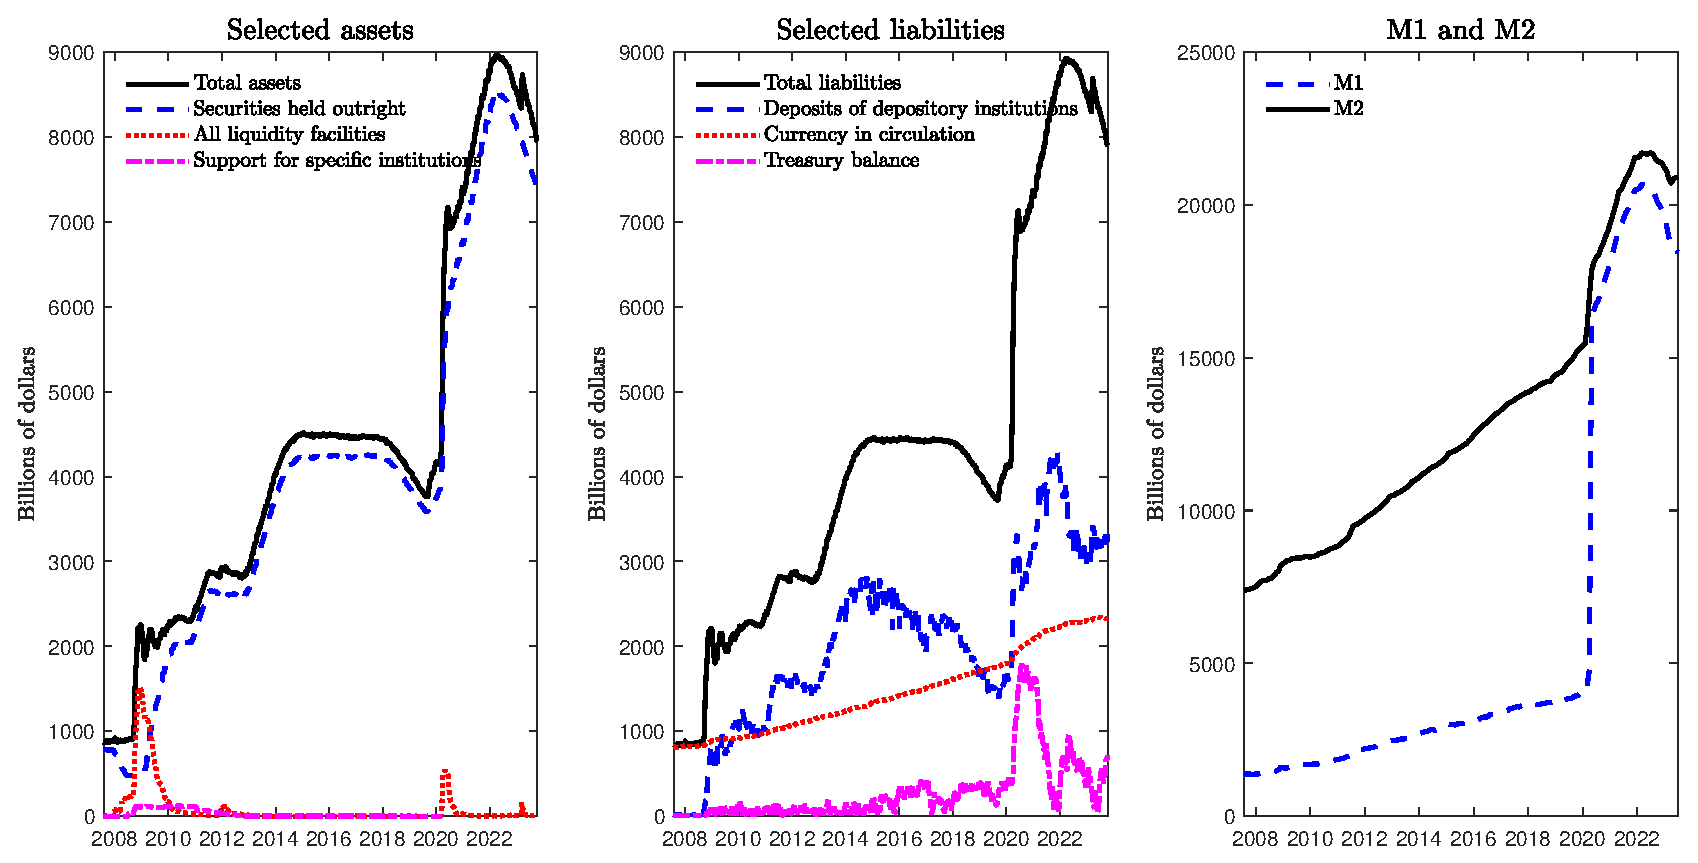
\includegraphics[width=0.85\linewidth]{Figures/Figure17.eps}
\caption{\tiny Selected assets of the Federal Reserve System (left
panel), selected liabilities (center panel), M1 and M2 (right panel).
Billions of dollars. Period: July 2007 - October 2023. \emph{Source: Fred Economic Data, St. Louis Fed.}}
\end{figure}
}
\end{frame}


% --- SLIDE 2: Balance Sheet Effects ---
\begin{frame}{Key Observations}
\small
\begin{itemize}
    \item \textbf{Assets:} Surge in long-term securities and liquidity facilities (e.g., Maiden Lane, Commercial Paper Funding).
    \vspace{0.2cm}
    \item \textbf{Liabilities:} Massive growth in deposits held by depository institutions.
    \vspace{0.2cm}
    \item \textbf{Monetary Aggregates:} Significant surge in M1 and M2, particularly during the pandemic.
\end{itemize}
\end{frame}

% --- SLIDE 3: Transmission Channels ---
\begin{frame}{Transmission Mechanisms: Two Views}
\small
\textcite{bernanke2022} mentions two contrasting views within the FOMC regarding the transmission mechanism of UMP.

\vspace{0.3cm}
\textbf{1. The Reserve Channel}
\begin{itemize}
    \item Expanding reserves induces banks to lend more, increasing liquidity and stimulating aggregate demand.
\end{itemize}

\vspace{0.3cm}

\textbf{2. The Portfolio Rebalancing Channel}
\begin{itemize}
    \item Central bank's purchases of long-term securities lower their yields. Investors reallocate portfolios toward other assets, lowering yields across the market.
\end{itemize}

\vspace{0.3cm}

This Section examines the portfolio-rebalancing channel via a frictionless financial-market model in which securities have only pecuniary benefits.


\end{frame}

% --- SLIDE 4a: Market Structure Setup --
\begin{frame}{Environment}
\small

\textbf{Stochastic Environment}
\begin{itemize}
    \item We extend the model discussed so far to include random preference shocks $\xi$ and output $Y$.
\end{itemize}

\vspace{0.2cm}

\textbf{Asset Characteristics}
\begin{itemize}
    \item The economy features both short-term ($B_S$) and long-term ($B_L$) debt.
    \item Market Clearing ensures:
    \begin{equation*}
        \underbrace{B_{S,t}^{F} = B_{S,t}+B_{S,t}^{C}}_{\text{Short-Term Bonds}} \quad \text{and} \quad \underbrace{B_{L,t}^{F} = B_{L,t}+B_{L,t}^{C},}_{\text{Long-Term Bonds}}
    \end{equation*}
    where the subscripts $F$ and $C$ denote Treasury issuance and central bank  holdings, respectively.
\end{itemize}
\end{frame}

% --- SLIDE 4b: Asset Returns Setup ---
\begin{frame}{Long-term Bonds}
\small

\textbf{Long-Term Bond Structure}
\begin{itemize}
    \item Long-term bonds with price $Q_t^L$ at time $t$ pay geometrically decaying coupons ($1, \delta, \delta^2...$) in subsequent periods.
    \item The realized return between $t-1$ and $t$ on long-term bonds $i_t^L$ is given by:
    \begin{equation*}
        1+i_{t}^{L} = \frac{1+\delta Q_{t}^{L}}{Q_{t-1}^{L}}
    \end{equation*}
\end{itemize}

\vspace{0.2cm}

\textbf{Key Implication}
\begin{itemize}
    \item Due to stochastic shocks, the long-term return may differ from the risk-free short rate ($i_{t}^{L} \neq i_{t-1}$).
    \item \textbf{Note:} The equilibrium is characterized as discussed so far, but now includes an additional asset-pricing condition for $Q_t^L$.
\end{itemize}
\end{frame}
% --- SLIDE 5: The Policy Experiment ---
\begin{frame}{Irrelevance of Open Market Operations: Experiment}
\small

\textbf{Experiment}
\vspace{0.1cm}
\begin{itemize}
    \item We assume that the central bank  \textbf{does not back} the Treasury.
    \item Consider a specific sequence of central bank  bond holdings:
    \begin{equation*}
        \left\{ \tilde{B}_{L,t}^{C}, \tilde{B}_{S,t}^{C} \right\}_{t=t_{0}}^{\infty}
    \end{equation*}
    \item \textbf{Intervention:} The central bank  alters this portfolio (e.g., purchasing more long-term bonds $\tilde{B}_{L,t}^{C}$) while keeping all other policy specifications unchanged.
    \item Does this change the equilibrium allocation and price level?
\end{itemize}
\end{frame}
% --- SLIDE 6: The Remittance Policy Condition ---
\begin{frame}{The Remittance Policy Condition}
\small

\textbf{Policy Specification}
\vspace{0.1cm}
\begin{itemize}
    \item Constant interest rate at $i_t = 1/\beta - 1$.
    \item Exogenous sequence of short and long-term bonds $\left\{ \tilde{B}_{L,t}^{C}, \tilde{B}_{S,t}^{C} \right\}_{t=t_0}^{\infty}$.
    \item We assume a specific remittance rule where the central bank  transfers a fixed real amount $\tau^C$ plus all variable returns:
    \begin{equation}
        \frac{T_{t}^{C}}{P_{t}}=(1-\beta )\tau ^{C}+\frac{i_{t-1}M_{t-1}+(i_{t}^{L}-i_{t-1})Q_{t-1}^{L}\tilde{B}_{L,t-1}^{C}}{P_{t}}. \label{Transfer}
    \end{equation}
    \item \textbf{Interpretation:} The central bank  rebates seigniorage from money issuance and any excess returns (or losses) from holding long-term assets directly to the Treasury.
\end{itemize}
\end{frame}
% --- SLIDE 7: Stochastic Equilibrium Condition ---
\begin{frame}{Intertemporal Resource Constraint}
\small

\textbf{Equilibrium Intertemporal Resource Constraint}
\vspace{0.1cm}
\begin{itemize}
    \item The relevant condition for determining prices is the stochastic version of the intertemporal resource constraint \eqref{KeyCB}, accounting for long-term debt holdings:

\begin{equation}
\frac{X_{t-1}+M_{t-1}-\tilde{B}_{S,t-1}^{C}-(1+i_{t}^{L})Q_{t-1}^{L}\tilde{B}_{L,t-1}^{C}}{P_{t}}=E_{t}\sum_{T=t}^{\infty }R_{t,T}\left( \frac{i_{T}}{1+i_{T}}\frac{M_{T}}{P_{T}}-\frac{T_{T}^{C}}{P_{T}}\right), \label{IBC-IR}
\end{equation}

where future real flows are discounted by the real stochastic discount factor $R_{t,T}$:
    \begin{equation*}
        R_{t,T} = \beta ^{T-t} \frac{\xi_{T}U_{c}(Y_{T})}{\xi _{t}U_{c}(Y_{t})}.
    \end{equation*}
\end{itemize}
\end{frame}

% --- SLIDE 8: Simplifying the Equilibrium ---
\begin{frame}{Simplifying the Equilibrium}
\small
\textbf{Deriving the Price Level Condition}
\begin{itemize}
    \item To simplify, we assume $\xi _{T}U_{c}(Y_{T})$ follows a martingale, i.e. $E_{t}\xi _{T}U_{c}(Y_{T})=\xi _{t}U_{c}(Y_{T})$ for each $T>t$. Substituting the transfer rule \eqref{Transfer} and the martingale property into \eqref{IBC-IR}, we obtain:
    \begin{equation*}
        \frac{N_{t-1}^{C}(1+i_{t-1})}{P_{t}}=\tau ^{C}.
    \end{equation*}
    \item Given the policy rate $1+i_{t}=1/\beta$, this simplifies to:
    \begin{equation}
        \frac{N_{t-1}^{C}}{P_{t}}=\beta \tau ^{C}, \label{CruxX}
    \end{equation}
where the net worth $N_{t}^{C}$ is defined as:
\begin{equation}
    N_{t}^{C}=Q_{t}^{L}\tilde{B}_{L,t}^{C}+\frac{\tilde{B}_{S,t}^{C}-X_{t}}{1+i_{t}}-M_{t}. \label{DefNW}
\end{equation}
\end{itemize}
\end{frame}
% --- SLIDE 9: Equilibrium Price Level Stability ---
\begin{frame}[label=Equilibrium]{Equilibrium Price Level Stability}
\small

\begin{itemize}
    \item Equation \eqref{CruxX} implies that $P_t$ depends on $N_{t-1}^C$ (predetermined) and parameters, making it \textbf{not contingent} on the current state. Using the stochastic Euler equation:
\end{itemize}

\vspace{0.2cm}

\textbf{Euler Equation} (stochastic version of $\ref{Euler-L}$)
\begin{equation*}
    \xi _{t}U_{c}(Y_{t})=\beta (1+i_{t})E_{t}\left\{ \frac{P_{t}}{P_{t+1}}\xi_{t+1}U_{c}(Y_{t+1})\right\}.
\end{equation*}

\vspace{0.2cm}

\begin{itemize}
    \item Using the martingale property of $\xi _{t}U_{c}(Y_{t})$, the result that $P_{t+1}$ is not state contingent, and the constant interest rate policy ($1+i_t = 1/\beta$), it follows that the price level is constant over time:
    \begin{equation*}
        P_t = P^* \quad \text{for all } t \ge t_0.
    \end{equation*}
    \item It can also be shown that \textbf{net worth} remains constant at $N_{t_o-1}$.
\end{itemize}
\centering  \hyperlink{Net}{\beamerbutton{Proof in Appendix}}
\end{frame}


% --- SLIDE 12: The Irrelevance Result ---
\begin{frame}{The Irrelevance Result}
\small

\textbf{Equilibrium Characterization}
\begin{itemize}
    \item With prices determined at $P_{t}=P^{\ast }$, the path of money supply is pinned down by the demand function \eqref{Money-L} for all $t \geq t_{0}$.
    \item The equilibrium is thus fully defined for the initial policy specification $\left\{ \tilde{B}_{S,t}^{C},\tilde{B}_{L,t}^{C}\right\}$.
\end{itemize}

\vspace{0.2cm}

\textbf{Policy Invariance}
\begin{itemize}
    \item Consider an alternative balance-sheet policy $\left\{ \bar{B}_{S,t}^{C},\bar{B}_{L,t}^{C}\right\}$ with active long-term bond purchases ($\bar{B}_{L,t}^{C}>0$).
    \item Since net worth is anchored at $N_{t_{0}-1}^{C}$, the price level $P^*$ and interest rate $i_t$ remain \textbf{unchanged}.
\end{itemize}

\vspace{0.1cm}

\textbf{Conclusion}
\begin{itemize}
    \item The equilibrium allocation is independent of whether the central bank  holds long-term securities.
\end{itemize}
\end{frame}
% --- SLIDE 13: The Intuition of Irrelevance ---
\begin{frame}{The Intuition of Irrelevance}
\small

\textbf{The Necessary Condition for Effectiveness}
\begin{itemize}
    \item For asset purchases to affect equilibrium prices, they must alter the \textbf{total wealth} (financial + human) of households.
    \item This is the same mechanism behind "Helicopter Money": creating a wealth effect to stimulate consumption.
\end{itemize}

\vspace{0.2cm}

\textbf{Why instead this Policy is Neutral}
\begin{itemize}
    \item The assumed remittance rule \eqref{Transfer} creates a closed loop that neutralizes risk:
    \begin{enumerate}
        \item \textbf{Risk Transfer:} If the central bank  incurs losses on risky assets that were before in the hand of households, it reduces transfers to the Treasury.
        \item \textbf{Fiscal Reaction:} To satisfy its solvency constraint, the Treasury must raise lump-sum taxes.
        \item \textbf{The Offset:} The private sector's reduced financial risk is perfectly offset by increased future tax liabilities. Total private \textbf{wealth} does not change.
    \end{enumerate}
\end{itemize}
\end{frame}

% --- SLIDE 14: The Passive Role of Reserves ---
\begin{frame}{The Mechanical Accommodation}
\small

\textbf{If prices don't move, what does?}
\begin{itemize}
    \item Constant nominal net worth ($N_t^C = N_{t_0-1}^C$) imposes the following identity:
    \begin{equation*}
        Q_{t}^{L}B_{L,t}^{C}+\frac{B_{S,t}^{C}}{1+i_{t}}-\frac{X_{t}}{1+i_{t}}-M_{t}=N_{t_{0}-1}^{C}
    \end{equation*}
    \item \textbf{Endogenous Adjustment:} Any change in the asset mix ($B_{S,t}^{C}$ vs. $B_{L,t}^{C}$) is perfectly accommodated by a variation in reserves ($X_t$), without any change in equilibrium prices $Q_{t}^{L}$, interest rate $i_t$ or money supply $M_t$.
\end{itemize}
\end{frame}

% --- SLIDE 15: Conclusion and Empirical Note ---
\begin{frame}{Conclusion: Limits of Pure Asset Swaps}
\small

\textbf{Summary of Irrelevance}
\begin{itemize}
    \item Massive asset purchases are ineffective if they function purely as asset swaps without an appropriate transfer policy to generate wealth effects.
    \item In the next section, we will see how changing the transfer policy restores effectiveness.
\end{itemize}

\vspace{0.4cm}

\hrule
\vspace{0.2cm}

\textbf{Note: Forward Guidance}
\begin{itemize}
    \item Our experiment held future interest rate policy constant.
    \item However, asset purchases may alter private sector expectations about \textit{future} rates (see \hyperref[ChapterFWG]{the Forward Guidance section}), and be indirectly effective through those changes.
\end{itemize}
\end{frame}

% --- SLIDE 16: Relevance of Open Market Operations ---
\begin{frame}{Relevance of Unconventional Open Market Operations}
\small
\begin{itemize}
    \item To break irrelevance, gains or losses must remain on the central bank's balance sheet.
    \item We assume a constant \textbf{real} remittance policy:
    \begin{equation*}
        \frac{T_{t}^{C}}{P_{t}}=(1-\beta )\tau ^{C}, \quad \text{with } \tau ^{C}>0.
    \end{equation*}
    \item Under this rule (and assuming constant $Y, \xi$), the budget constraint \eqref{IBC-IR} implies:
    \begin{equation}
        L(Y,\beta ^{-1}-1)+\frac{N_{t-1}^{C}+\Psi _{t}^{C}}{P_{t}}=\tau ^{C}. \label{Seinior}
    \end{equation}
\end{itemize}
\end{frame}
% --- SLIDE 17: Portfolio Composition and Price Determination ---
\begin{frame}{Portfolio Composition and Price Determination}
\small

\textbf{Impact of Unconventional Interventions}
\begin{itemize}
    \item Consider an initial equilibrium where the central bank  holds only short-term, risk-free assets ($B_{L,t}^{C}=0$).
    \item Under this specification, profits $\Psi_t^C$ are independent of long-term bond returns.
    \item The central bank  expands its balance sheet or substitutes assets to hold long-term securities ($B_{L,t}^{C} > 0$).
    \item A negative shock to bond returns reduces profits. To satisfy the budget constraint \eqref{Seinior} given fixed real remittances $\tau^C$, the price level must adjust downward.
    \item \textbf{Conclusion:} Under the specified remittances policy, the asset composition of the central bank  becomes a determinant of the equilibrium price level.
\end{itemize}
\end{frame}

% --- SLIDE 18: Sustainability of the Interest Rate Peg ---
\begin{frame}{Sustainability of the Interest Rate Peg}
\small

\textbf{Breakdown of the Peg}
\begin{itemize}
    \item What happens if the central bank incurs \textit{substantial} losses on its risky portfolio?
    \vspace{0.25em}
    \item If these losses are large enough to make the left-hand side of the solvency condition \eqref{Seinior} negative, the equilibrium breaks down.
     \vspace{0.25em}
    \item Under the constant remittance policy $\tau^C$, an interest rate peg of $i = 1/\beta - 1$ (implying zero net inflation) becomes \textbf{infeasible}.
     \vspace{0.25em}
    \item \textbf{Implication:} Without a fiscal recapitalization, the central bank must change policy—abandoning the simple peg and altering its future interest rate trajectory.
\end{itemize}
\end{frame}


% --- SLIDE 19: Reflation via Seigniorage ---
\begin{frame}{Reflation via Seigniorage}
\small

\textbf{Restoring Equilibrium}
\begin{itemize}
    \item The central bank could target a new nominal interest rate $i = \Pi/\beta - 1$, consistent with a positive inflation target $\Pi > 1$.
    \item The intertemporal budget constraint is modified to include \textbf{seigniorage revenues} as the balancing mechanism:
    \begin{equation*}
        \underbrace{\frac{\Pi -\beta }{\Pi (1-\beta )}L\left( Y,\frac{\Pi }{\beta }-1\right)}_{\text{Seigniorage Revenue}} + \frac{N_{t-1}^{C}+\Psi _{t}^{C}}{P_{t}}=\tau ^{C}.
    \end{equation*}
    \item \textbf{Mechanism:} A large negative $\Psi_t^C$ (loss) is absorbed by an increase in inflation $\Pi$. This generates the seigniorage necessary to cover the shortfall, effectively "reflating" the economy.
\end{itemize}
\end{frame}

% --- SLIDE 20: Real-World Remittance Policies ---
\begin{frame}{Real-World Remittance Policies (e.g., The Fed)}
\small

\textbf{Beyond Constant Remittances}
\begin{itemize}
    \item In practice, policies are more complex. For instance, the US Federal Reserve rebates profits during normal times but \textbf{halts remittances} during periods of loss.
    \item Losses are accumulated as a "deferred asset" and must be recovered before transfers resume.
\end{itemize}

\vspace{0.2cm}

\textbf{Formalizing the Rule}
\begin{itemize}
    \item If we assume a target nominal net worth $\bar{N}^{C}$, the rule can be written as:
    \begin{equation*}
        T_{t}^{C} =
        \begin{cases}
            \max (\Psi _{t}^{C},0) & \text{if } N_{t-1}^{C}\geq \bar{N}^{C} \\
            0 & \text{otherwise}
        \end{cases}
    \end{equation*}
    \item \textbf{Result:} Under this asymmetric rule, open market operations remain \textbf{relevant} (affecting prices) if losses are large enough.
\end{itemize}
\end{frame}

% --- SLIDE 21: Summary: The Wealth Effect Channel ---
\begin{frame}{Summary: Helicopter Money \& UMP}
\small

\textbf{Comparing Policy Tools}
\begin{itemize}
    \item Our analysis of Helicopter Money and UMP converges on a single insight: effectiveness depends on generating \textbf{wealth effects}.
\end{itemize}

\vspace{0.3cm}

\textbf{Mechanisms of Wealth Transfer}
\begin{itemize}
    \item \textbf{Helicopter Money:} Effectiveness relies on a \textit{direct} fiscal transfer to households that is not negated by future tax increases.
    \item \textbf{UMP / QE:} Effectiveness relies on an \textit{implicit} transfer. Asset purchases work only if the associated risk/wealth transfer behaves like a fiscal injection (i.e., central bank  losses are not taxed back).
\end{itemize}
\end{frame}

% --- SECTION TITLE SLIDE ---
\section{Forward Guidance}

% --- SLIDE 22: Beyond Static Policy Analysis ---
\begin{frame}[label=ChapterFWG]{Beyond Static Policy Analysis}
\small

\textbf{Limitations of Previous Analysis}
\begin{itemize}
    \item Our analysis so far assumed a \textbf{perfect alignment} between the duration of the exogenous negative shock and ZLB policy.
    \item This simplification obscured the importance of interest rate policy \textit{during} and \textit{after} the crisis. The duration of zero interest rate policy beyond the occurrence of the shock can be an instrument of policy.
    \item Explicitly offering guidance on the future path of the policy rate is known as \textit{Forward Guidance}.
\end{itemize}
\end{frame}

% --- SLIDE 24: Forward Guidance at the Zero Lower Bound ---
\begin{frame}{Forward Guidance at the Zero Lower Bound}
\small

\textbf{Strategic Relevance in a Liquidity Trap}
\begin{itemize}
    \item While Forward Guidance is a standard tool of monetary policy, it becomes critical when the short-term nominal interest rate binds at the Zero Lower Bound (ZLB).
    \item In a dynamic setting, the duration of the zero-interest rate policy is not strictly determined by the duration of the exogenous negative shock.
    \item Instead, the duration of the ZLB period becomes a \textbf{strategic choice variable} for the policymaker.
    \item \textbf{Mechanism:} Committing to keep rates at zero \textit{longer} than the shock persists generates the inflationary expectations necessary to lower real interest rates and stimulate demand.
\end{itemize}
\end{frame}

% --- SLIDE 25: Optimal Policy Constraints ---
\begin{frame}{Optimal Policy Constraints and the ZLB}
\small

\textbf{Revisiting Optimal Policy}
\begin{itemize}
    \item In the standard optimal policy analysis (Chapter 7), the Aggregate Demand equation was \textbf{not} a binding constraint.
    \item The framework implicitly assumed that the nominal interest rate $\hat{\imath}_{t}$ could freely adjust to track the natural rate $r_t^e$ and the output gap $x_t$:
    \begin{equation*}
        \hat{\imath}_{t}=r_{t}^{e}-(\sigma ^{-1}-\theta ^{-1})(1-\gamma _{1})x_{t}.
    \end{equation*}
    \item \textit{Validity Condition:} This solution remains valid only if shocks to $r_t^e$ are sufficiently small, such that $\hat{\imath}_{t} \ge 0$ is naturally satisfied.
    \item In the presence of large negative shocks to the real rate $r_{t}^{e}$, the unconstrained solution violates the zero lower bound.
    \item Consequently, the optimization problem must be reformulated to explicitly incorporate:
    \begin{enumerate}
        \item The Aggregate Demand (AD) equation as a binding restriction.
        \item The Zero Lower Bound (ZLB) inequality constraint, $\hat{\imath}_{t} \geq 0$.
    \end{enumerate}
\end{itemize}
\end{frame}
% --- SLIDE 26: The Constrained Lagrangian Formulation ---
\begin{frame}{The Constrained Lagrangian Formulation}
\small

\textbf{Augmented Lagrangian from Chapter 7}
\footnotesize
\begin{equation*}
\begin{aligned}
\mathcal{L}_{t_{0}} &= E_{t_{0}} \sum_{t=t_{0}}^{\infty } \beta^{t-t_{0}} \Bigg[ \underbrace{\frac{1}{2}( \hat{Y}_{t}-\hat{Y}_{t}^{e}) ^{2} + \frac{1}{2}\frac{\theta }{\kappa }(\pi _{t}-\pi ) ^{2}}_{\text{Loss Function}} \\
&\quad + \underbrace{\varphi _{t}\left[ (\hat{Y}_{t}-\hat{Y}_{t}^{e})-(\hat{Y}_{t+1}-\hat{Y}_{t+1}^{e})+\sigma ( \hat{\imath}_{t}-(\pi _{t+1}-\pi )-r_{t}^{e}) \right]}_{\text{AD Constraint}} \\
&\quad + \underbrace{\lambda _{t}\left[ (\pi _{t}-\pi )-\kappa (\hat{Y}_{t}-\hat{Y}_{t}^{e})-\upsilon _{t}-\beta (\pi _{t+1}-\pi )\right]}_{\text{AS Constraint}} \Bigg] \\
&\quad \underbrace{-\varphi _{t_{0}-1}\beta ^{-1}(\hat{Y}_{t_{0}}-\hat{Y}_{t_0}^{e})-\varphi _{t_{0}-1}\beta ^{-1}\sigma (\pi _{t_{0}}-\pi )-\lambda _{t_{0}}(\pi _{t_{0}}-\pi )}_{\text{Initial Conditions (Timeless perspective constraints)}}
\end{aligned}
\end{equation*}

\vspace{0.2cm}
\scriptsize
\centering\textit{Note: All variables and notations follow the definitions established in Chapter 7.}
\end{frame}
% --- SLIDE 27: Optimality Conditions ---
\begin{frame}{Optimality Conditions}
\small

\textbf{First-Order Conditions (FOCs)}
\begin{itemize}
    \item Minimizing the Lagrangian with respect to inflation $\pi_t$ and output gap $\hat{Y}_{t}$ yields:
    \begin{equation}
        \theta (\pi _{t}-\pi )-\beta ^{-1}\sigma \kappa \varphi _{t-1}+\kappa \lambda _{t}-\kappa \lambda _{t-1}=0 \label{FOCzl1}
    \end{equation}
    \begin{equation}
        (\hat{Y}_{t}-\hat{Y}_{t}^{e})+\varphi _{t}-\beta ^{-1}\varphi _{t-1}-\kappa \lambda _{t}=0 \label{FOCzl2}
    \end{equation}
\end{itemize}

\vspace{0.2cm}

\textbf{The Kuhn-Tucker Condition}
\begin{itemize}
    \item The non-negativity constraint on the nominal interest rate ($i_t \ge 0$) implies the complementarity condition:
    \begin{equation*}
        i_{t} \cdot \varphi _{t} = 0 \quad \text{and} \quad \varphi_t \ge 0
    \end{equation*}
    \item $\varphi_t > 0$ only when the ZLB is binding ($i_t = 0$). If not binding ($\varphi_t = 0$), we recover the standard solution of Chapter 7.
\end{itemize}
\end{frame}

% --- SLIDE 28: A Dynamic Price-Level Target ---
\begin{frame}{Synthesizing a Target Rule}
\small

\textbf{Defining the "Adjusted Price"}
\begin{itemize}
    \item Combining the FOCs to express the optimal policy in terms of the target variable $\tilde{p}_{t}$ be the "adjusted price level" (price level + weighted output gap):
    \begin{equation*}
        \tilde{p}_{t} = p_{t} + \theta ^{-1}(\hat{Y}_{t}-\hat{Y}_{t}^{e})
    \end{equation*}
\end{itemize}

\vspace{0.2cm}

\textbf{The Targeting Strategy}
\begin{itemize}
    \item The central bank  aims to set $\tilde{p}_{t}$ equal to a target $\bar{p}_{t}^{\ast }$.
    \item \textbf{If feasible ($i_t > 0$):} The target is met perfectly: $\tilde{p}_{t} = \bar{p}_{t}^{\ast }$.
    \item \textbf{If infeasible ($i_t = 0$):} The actual $\tilde{p}_{t}$ falls below $\bar{p}_{t}^{\ast }$, and the gap accumulates in the target variable.
\end{itemize}
\end{frame}

% --- SLIDE 29: Evolution of the Target ---
\begin{frame}{Optimal Policy}
\small

\textbf{Law of Motion for the Target $\bar{p}_{t}^{\ast }$}
\begin{itemize}
    \item The target $\bar{p}_{t}^{\ast }$ is updated following the law of motion:
    \begin{equation*}
        \bar{p}_{t+1}^{\ast }=\pi +\bar{p}_{t}^{\ast }+\beta ^{-1}(1+\kappa \sigma )(\bar{p}_{t}^{\ast }-\tilde{p}_{t})-\beta ^{-1}(\bar{p}_{t-1}^{\ast }-\tilde{p}_{t-1}).
    \end{equation*}
    \item This relation is obtained by eliminating the Lagrange multipliers and defining the target as $\bar{p}_{t}^{\ast }\equiv \varphi _{t}+\tilde{p}_{t}$.
    \item The target is adjusted upward during periods in which it is not achieved ($\bar{p}_{t}^{\ast }>\tilde{p}_{t}$) and the zero-lower bound is tight. This increase in the target during the liquidity trap works to push up inflation expectations.
    \item Conversely, when the zero-lower bound is no longer binding, the price target decreases at that moment, as captured by the last term on the RHS.
    \item Under normal conditions of a positive nominal interest rate: $\tilde{p}_{t}=\bar{p}_{t}^{\ast }$ and the target simply grows at the rate $\pi$ (as discussed in Chapter 7).
\end{itemize}
\end{frame}
% --- SLIDE 30: The Suboptimal Benchmark ---
\begin{frame}{Comparison: The Suboptimal Policy}
\small

\begin{itemize}
    \item Consider a central bank  that\textbf{ never adjusts} its target price level trajectory, even after missing it.
    \item The target follows the standard path $\tilde{p}_{t+1}^{\ast }=\pi +\tilde{p}_{t}^{\ast }$ (as in Chapter 7).
\end{itemize}

\vspace{0.2cm}

\textbf{Implementation and Limitation}
\begin{itemize}
    \item \textbf{Implementation:} If feasible ($i_t > 0$), the target is met ($\tilde{p}_{t} = \tilde{p}_{t}^{\ast }$). If infeasible ($i_t = 0$), the central bank  simply accepts the deviation.
    \item \textbf{The Flaw:} While optimal \textit{outside} the ZLB, this strategy is suboptimal when binding because it fails to "catch up" to the lost price level trajectory.
\end{itemize}
\end{frame}

% --- SLIDE 31: Figure 18 (Simulation Results) ---
\begin{frame}{Simulation: Optimal vs. Suboptimal Policy}
\small
{
\setbeamertemplate{caption}{\raggedright\insertcaption\par}
\begin{figure}[t]
\centering
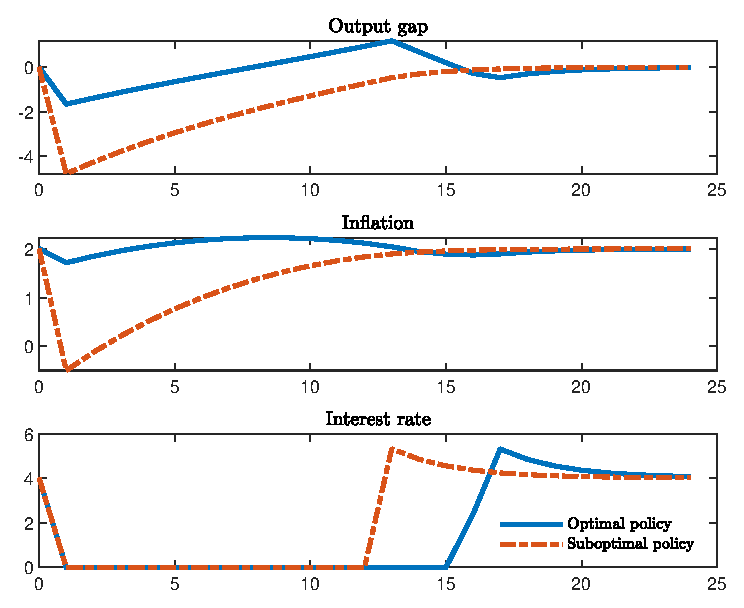
\includegraphics[width=0.53\linewidth]{Figures/Figure18.eps}
\caption{\tiny Responses of output gap, inflation, and interest rate to a negative shock to the natural rate of interest (duration: 12 quarters). \textbf{Solid Line:} Optimal Policy. \textbf{Dashed Line:} Suboptimal Policy (Standard Targeting). Variables are in \%. Rates are annualized. Parameters are calibrated as in Chapter 7.}
\end{figure}
}
\end{frame}

% --- SLIDE 32: Interpreting the Simulation ---
\begin{frame}{Key Result: "Lower for Longer"}
\small

\textbf{The Optimal Response}
\begin{itemize}
    \item The economy is hit by a severe negative shock: the natural rate falls to $-4\%$ (annualized) for 12 quarters.
    \item A suboptimal (standard) policy would keep rates at zero for exactly 12 quarters, rising immediately as the shock subsides.
    \item The optimal policy keeps the interest rate at zero for 15 quarters.
    \item This captures the essence of \textit{Forward Guidance}: By committing to keep rates low even after the natural rate recovers, the central bank  generates the inflation expectations needed to stimulate the economy \textit{today}.
    \item \textbf{Implication:} Another way to communicate Forward Guidance is to explicitly promise \textbf{higher inflation than the target} (overshooting) after the negative shock ends.
\end{itemize}
\end{frame}

% --- SLIDE 33: Evolution of Communication ---
\begin{frame}{Forward Guidance in Practice}
\small
 Central Bank's have progressively adopted more specific forms of guidance to implement these theoretical insights:

\begin{enumerate}
    \item \textbf{Qualitative (Fed 2003):} "Policy accommodation can be maintained for a \textit{considerable period}."
    \item \textbf{Extended (Fed 2008):} Rates will stay low for an "\textit{extended period of time}."
    \item \textbf{Time-Contingent (Fed 2011):} Specific dates provided (e.g., rates will stay low "at least through mid-2013").
    \item \textbf{State-Contingent (Fed 2012):} Lift-off linked to specific economic outcomes (unemployment $> 6.5\%$ and stable inflation), rather than calendar dates.
\end{enumerate}
\end{frame}
% --- SLIDE 35: Figure 19 (Price Level Path) ---
\begin{frame}{Price Level Dynamics}
\small
{
\setbeamertemplate{caption}{\raggedright\insertcaption\par}
\begin{figure}[t]
\centering
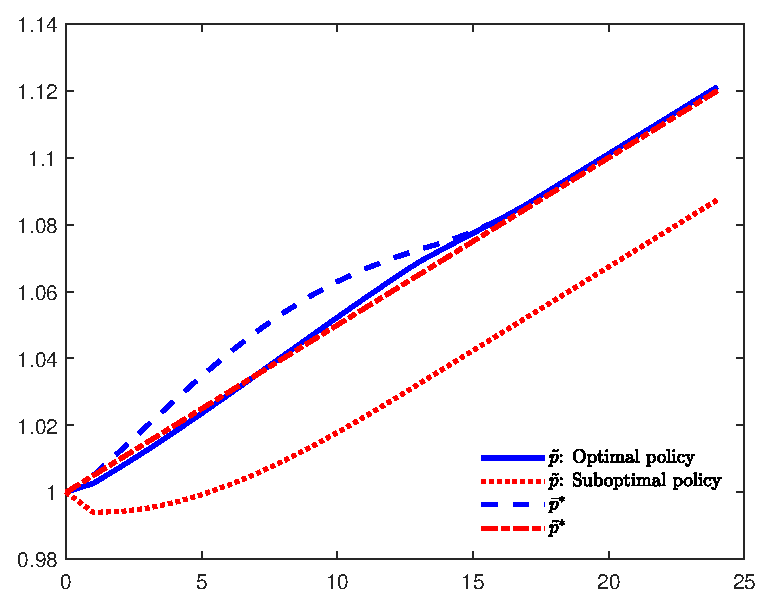
\includegraphics[width=0.55\linewidth]{Figures/Figure19.eps}
\centering\caption{\tiny Evolution of the adjusted price level $\tilde{p}_{t}$ under Optimal Policy vs. Suboptimal Policy. The graph compares the realized path against the optimal target $\bar{p}_{t}^{\ast }$ and the suboptimal target $\tilde{p}_{t}^{\ast }$.}
\end{figure}
}
\end{frame}
% --- SLIDE 36: History Dependence vs. Bygones ---
\begin{frame}{Price Level under Optimal vs. Suboptimal Policies}
\small

\textbf{Suboptimal Policy: “Bygones are bygones”}
\begin{itemize}
    \item The adjusted price level $\tilde{p}_{t}$ (dotted red line) falls sharply during the initial liquidity trap. Once the constraint lifts, the price level resumes growing at the standard 2\% rate, but the permanent shortfall is accepted — the central bank  ignores past misses.
\end{itemize}

\vspace{0.3cm}

\textbf{Optimal Policy: History Dependence}
\begin{itemize}
    \item The optimal path $\tilde{p}_{t}$ (solid blue line) attempts to catch up with the target $\bar{p}_{t}^{\ast}$ (dashed blue line). To achieve this catch-up, inflation must eventually exceed 2\%.
\end{itemize}
\end{frame}

% --- SLIDE 37: Recent Policy Framework Updates ---
\begin{frame}{Policy Framework Reviews}
\small
\begin{itemize}
    \item The implications of this New-Keynesian model directly support the strategic reviews conducted by major central banks.
\end{itemize}

\vspace{0.2cm}

\textbf{Federal Reserve (2020 Review)}
\begin{itemize}
    \item Adopted \textbf{Average Inflation-Targeting}.
    \item Explicitly acknowledges that periods of inflation persistently below 2\% should be followed by periods of inflation \textit{above} the target.
\end{itemize}

\vspace{0.2cm}

\textbf{European Central Bank  (2021 Review)}
\begin{itemize}
    \item Replaced "below but close to 2\%" with \textbf{a symmetric 2\% target}.
    \item Explicitly recognizes the asymmetry imposed by the effective lower bound. This strategy allows for "a temporary period during which inflation moderately exceeds the target", consistent with the optimal policy prescription.
\end{itemize}
\end{frame}

% --- SECTION TITLE SLIDE ---
\section{Managing the Central Bank's Reserves}
\label{CH-Reserves}

% --- SLIDE 38: Beyond Interest Rate Policy ---
\begin{frame}{Beyond Interest Rate Policy: Asset Purchases}
\small

\textbf{The Challenge of "Tapering"}
\begin{itemize}
    \item While Forward Guidance clarifies the future path of interest rates, the path and timing of asset purchases (QE) represent a distinct policy dimension.
    \item \textbf{Historical Context:} The "Taper Tantrum" of June 2013 illustrates the market's sensitivity to these flows.
    \item When the Federal Reserve signaled a potential reduction in the pace of asset purchases ("tapering"), markets reacted with panic, triggering a sharp spike in U.S. Treasury yields.
\end{itemize}
\end{frame}

% --- SLIDE 39: The Mechanics of QE: The Reserves Channel ---
\begin{frame}{The Mechanics of QE: The Reserves Channel}
\small

\textbf{Alternative Transmission Mechanisms}
\begin{itemize}
    \item To analyze QE theoretically, we focus on the \textbf{Reserves Channel} (the "Monetarist View"), where an increase in central bank  reserves is supposed to trigger liquidity creation via financial intermediaries, thereby stimulating aggregate demand.
    \item We use the New-Keynesian framework with financial frictions introduced in Chapter 8.
    \item In this setup, reserves are not neutral. They provide distinct non-pecuniary benefits to intermediaries by relaxing collateral or regulatory constraints.
\end{itemize}
\end{frame}
% --- SLIDE 40: Optimal Liquidity Policy and Satiation ---
\begin{frame}{Optimal Liquidity Policy and Satiation}
\small

\textbf{Applying the ZLB to the Banking Model}
\begin{itemize}
    \item We apply the zero-lower bound constraint to the optimal policy problem from Chapter 8. Strikingly, the optimal liquidity policy remains \textbf{unchanged} relative to the unconstrained case. 
    \item The central bank  should supply reserves up to the point of \textbf{satiating} the liquidity needs of the economy.
    \item Once the economy reaches the satiation level, further increases in central bank  reserves are \textbf{irrelevant}.
    \item \textbf{Conclusion:} Reserve policy is impactful only when satiation is \textit{not} yet reached.
\end{itemize}
\end{frame}

% --- SLIDE 41: Liquidity with Distortionary Taxation ---
\begin{frame}{Liquidity with Distortionary Taxation}
\small

\textbf{The Assumption of Costly Liquidity}
\begin{itemize}
    \item The role and dynamic of liquidity become more significant when it is costly to vary it, such as in a context in which lump-sum taxes are not available.
    \item We reconsider the model of Chapter 8 under the assumption that the only available tax is the distortionary tax on firm's revenues ($\tau$).
    \item Under this assumption, the overall supply of government liquidity, $B_{t-1}^{g}$, is directly related to the distortionary tax through the intertemporal resource constraint of the economy.
\end{itemize}
\end{frame}

% --- SLIDE 42: The Intertemporal Resource Constraint ---
\begin{frame}{The Intertemporal Resource Constraint}
\small

\begin{itemize}
    \item The resource constraint linking liquidity and fiscal variables, replacing (8.19), is given by:
\end{itemize}
\footnotesize
\begin{equation}
\frac{(1+i_{t-1}^{X})B_{t-1}^{g}}{P_{t}}=E_{t}\left\{ \sum_{T=t}^{\infty
}R_{t,T}\left[ \tau _{T}Y_{T}-Tr_{T}+\frac{i_{T}-i_{T}^{X}}{1+i_{T}}\frac{%
B_{T}^{g}}{P_{T}}\right] \right\}.  \label{IBCGbis}
\end{equation}
\vspace{0.2cm}
\small
\textbf{Variable Definitions}
\begin{itemize}
    \item $R_{t,T}$ is the stochastic discount factor for real income.
    \item $i^X$ is the policy rate.
    \item $i$ is the market nominal interest rate.
    \item $Tr$ is an exogenous non-negative transfer.
    \item $\tau$ is the distortionary tax on firms' revenues.
\end{itemize}
\end{frame}
% --- SLIDE 43: Welfare Implications of Costly Liquidity ---
\begin{frame}{Welfare Implications of Costly Liquidity}
\small

\textbf{The Trade-off}
\begin{itemize}
    \item Supplying liquidity generates taxation-related distortions that can negatively impact overall welfare.
    \item As previously discussed in Chapter 8, the optimal supply of liquidity is therefore deemed to be \textbf{below the satiation level}.
    \item Increasing liquidity beyond this point would necessitate significant distortions in taxation that outweigh the benefits of additional liquidity services.
    \item We analyze the optimal government stabilization problem using a linear-quadratic approach.
    \item The approximations are centered around an optimal steady state where inflation is at the target level, but liquidity remains below the satiation threshold.
\end{itemize}
\end{frame}

% --- SLIDE 44: The Quadratic Loss Function ---
\begin{frame}{The Quadratic Loss Function}
\small
\begin{itemize}
    \item The quadratic welfare-based loss function takes the following form:
\end{itemize}

\footnotesize
\begin{equation}
    L_{t_{0}}^{CB}=E_{t_{0}}\sum_{t=t_{0}}^{\infty }\beta ^{t-t_{0}}\left\{ \frac{1}{2}\Lambda _{x}x_{t}^{2} + \frac{1}{2}\Lambda _{\pi }(\pi _{t}-\pi )^{2} +\underbrace{\frac{1}{2}\Lambda _{d}\hat{d}_{t}^{2}}_{\text{Real Liquidity}} \right\} \label{Loss-Text}
\end{equation}
\vspace{0.2cm}
\small
\begin{itemize}
    \item The parameters $\Lambda _{x}$, $\Lambda _{\pi }$, and $\Lambda _{d}$ are positive weights derived from structural parameters (\cite{benigno2022}).
    \item The policymaker aims to minimize the deviation of the output gap ($x$), inflation ($\pi$), and real liquidity (deposits, $\hat{d}$) from their steady-state values, given the supply, demand and resource constraint.
    \item The analysis considers two stochastic disturbances: the preference shock $\xi$ and the exogenous transfer $Tr$.
\end{itemize}
\end{frame}
% --- SLIDE 45: Modified Supply Constraint ---
\begin{frame}{Modified Supply Constraint}
\small

\textbf{The Aggregate Supply (AS) Equation}
\begin{itemize}
    \item The optimal policy problem is subject to a modified Phillips Curve (relative to Chapter 8):
\end{itemize}

\footnotesize
\begin{equation*}
    (\pi _{t}-\pi )=\kappa \bigg[ x_t + \underbrace{\psi _{\tau }(\tilde{\tau}_{t}-\tilde{\tau}_{t}^{\ast })}_{\text{Tax Distortion Effect}} \bigg] + \beta E_{t}(\pi _{t+1}-\pi )
\end{equation*}

\vspace{0.2cm}
\small
\textbf{Interpretation}
\begin{itemize}
    \item This equation accounts for the time-varying supply-side effects of the distortionary tax on firms' revenue ($\psi _{\tau } > 0$).
    \item $\tilde{\tau}_{t} = \tau _{t}-\tau$ represents the deviation of the tax rate from its steady state.
    \item $\tilde{\tau}_{t}^{\ast }$ represents the "efficient" tax deviation—a combination of shocks such that if $\tilde{\tau}_{t} = \tilde{\tau}_{t}^{\ast }$, the tax wedge is neutralized, allowing output and inflation to be stabilized at their targets.
\end{itemize}
\end{frame}% --- SLIDE 46: Modified Demand and Fiscal Constraints ---
\begin{frame}{Modified Demand and Fiscal Constraints}
\small

\textbf{Aggregate Demand (AD) with Banking Frictions}
\begin{equation}
  x_{t}=\nu _{\rho }E_{t}x_{t+1}-\sigma \nu _{\rho }(\hat{\imath}_{t}^{X}-E_{t}(\pi _{t+1}-\pi )-r_{t}^{e}) + d_{y}^{-1}(1-\nu _{\rho })\hat{d}_{t} \label{ADfinal}
\end{equation}
\vspace{-0.2cm}
\footnotesize
\begin{itemize}
    \item $r_{t}^{e}$ is the \textbf{constrained efficient real rate} (function of shocks).
    \item Parameters $\nu_{\rho}, \sigma, d_{y}$ are positive.
\end{itemize}

\vspace{0.1cm}
\small
\textbf{The Linearized Resource Constraint \eqref{IBCGbis}}
\begin{equation}
\begin{split}
  \hat{d}_{t-1}-(\pi _{t}-\pi )-\sigma ^{-1}x_{t}+(\hat{\imath}_{t-1}^{X}-r_{t-1}^{e}) = \quad\quad\quad \\
   -\mathrm{f}_{t} + E_{t}\sum_{T=t}^{\infty }\beta ^{T-t}\Big[ b_{x}x_{T}+b_{\tau }(\tilde{\tau}_{T}-\tilde{\tau}_{T}^{\ast })+b_{d}\hat{d}_{T} \Big]
\end{split}
\label{IBCGlin}
\end{equation}

\end{frame}

% --- SLIDE 47: Feasibility and Fiscal Stress ---
\begin{frame}{Feasibility and Fiscal Stress}
\small

\textbf{\textcite{eggertsson2004}: Fiscal Stress ($\mathrm{f}_{t}$)}
\begin{itemize}
    \item The variable $\mathrm{f}_{t}$ measures the \textbf{"Fiscal Stress"}: the extent to which full stabilization of targets ($x, \pi, d$) is incompatible with the government's intertemporal budget constraint.
    \item If $\mathrm{f}_{t} > 0$, the government lacks the fiscal space for a constrained optimal outcome.
\end{itemize}

\vspace{0.4cm}

\textbf{Feasibility Conditions}
\begin{itemize}
    \item \textbf{Ideal Case ($\mathrm{f}_{t}=0$):} It is feasible to reach all three targets provided the natural rate does not violate the ZLB. In this case, the policy rate tracks the natural rate perfectly: $\hat{\imath}_{t}^{X}=r_{t}^{e}$.
    \item \textbf{The ZLB Constraint:} However, if $r^{e}$ falls substantially, the ZLB binds ($i^{X} \ge 0$). Even without fiscal stress, this forces a trade-off between stabilizing the relevant variables.
\end{itemize}

\end{frame}
\begin{frame}{Comparison of Policy Simulations}
\small
{
\setbeamertemplate{caption}{\raggedright\insertcaption\par}
\begin{figure}[t]
\centering
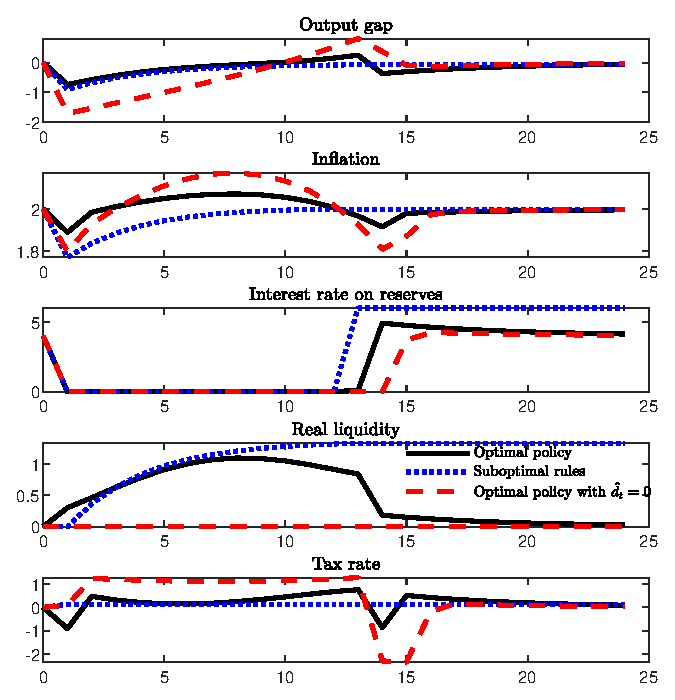
\includegraphics[width=0.42\linewidth]{Figures/Figure20.eps}
\centering\caption{\tiny Comparison between the optimal policy, a sub‑optimal policy, and the optimal policy with no adjustments to liquidity.}
\end{figure}
}
\end{frame}
% --- SLIDE 49: Defining the Policy Benchmarks ---
\begin{frame}{Suboptimal Policies}
\small

\textbf{Benchmark 1: Constrained Inflation Targeting}
\begin{itemize}
    \item \textbf{Monetary Rule:} Strictly targets inflation ($\pi _{t}=\pi$). If the target requires $i_t < 0$, the rate hits the zero floor.
    \item \textbf{Fiscal Role:} \textit{Passive.} Maintains a constant expected tax gap consistent with solvency; does not react to the crisis.
\end{itemize}

\vspace{0.4cm}

\textbf{Benchmark 2: Constant Liquidity Policy}
\begin{itemize}
    \item \textbf{Objective:} Isolates the optimal response \textbf{without} active liquidity management.
    \item \textbf{Fiscal Rule:} Adjusts taxes purely to stabilize real liquidity at the steady state ($\hat{d}_t = 0$).
    \item \textbf{Monetary Rule:} Minimizes the loss function subject to this liquidity-neutral fiscal constraint.
\end{itemize}
\end{frame}

% --- SLIDE 50: Analysis of Policy Outcomes ---
\begin{frame}{Analysis: Optimal vs. Suboptimal Outcomes}
\small

\textbf{The Cost of Suboptimal Policies}
\begin{itemize}
    \item \textbf{Deep Contraction:} Significant welfare losses characterized by a sharp drop in output and inflation persistently below target.
    \item \textbf{Premature Liftoff:} The policy rate rises from the ZLB \textbf{exactly} when the shock vanishes. This lack of commitment fails to stimulate expectations.
\end{itemize}

\vspace{0.4cm}

\textbf{The Gains from Optimization}
\begin{itemize}
    \item \textbf{Stabilization:} Optimal policy leverages multiple tools to keep inflation close to target and output variations moderate.
    \item \textbf{Mechanism:} It creates a "history-dependent" path that suboptimal rules ignore.
\end{itemize}

\end{frame}

% --- SLIDE 51: Feature 1: Optimal Duration and Liftoff ---
\begin{frame}{Feature 1: Optimal Duration and Liftoff}
\small

\textbf{Forward Guidance: “Lower for longer”}
\begin{itemize}
    \item As discussed in the Forward Guidance section, the optimal policy keeps the interest rate at zero for longer than the duration of the shock itself.
    \item Although the optimal policy remains low longer than a \textit{standard} rule, it lifts off \textit{earlier} than under a \textit{constant liquidity policy}.
    \item This highlights the benefits and complementarities of actively managing reserves and liquidity.
\end{itemize}

\end{frame}


% --- SLIDE 52: Feature 2: Dynamics of Asset Purchases ---
\begin{frame}{Feature 2: Dynamics of Asset Purchases (QE)}
\small

\textbf{Reversibility vs. Permanence}
\begin{itemize}
    \item \textbf{Expansion:} Liquidity is injected aggressively at the start of the trap, peaking just before the shock ends.
    \item \textbf{Normalization:} A sharp withdrawal occurs precisely at lift‑off, followed by a gradual return to the steady state as the balance sheet is fully unwound (reversibility).
    \item \textbf{Sub‑optimal policy:} A \emph{permanent} accumulation of public debt increases long‑run tax distortions.
\end{itemize}
\end{frame}


% --- SLIDE 53: Feature 3: Fiscal Coordination ---
\begin{frame}{Feature 3: Optimal Fiscal Coordination}
\small

\begin{itemize}
    \item Optimal policy requires the distortionary tax rate ($\tau$) to adjust at two critical moments:
\end{itemize}

\vspace{0.2cm}

\textbf{1. At the Onset (Producing Fiscal Stimulus)}
\begin{itemize}
    \item Taxes are \textbf{lowered} to stimulate the rise in government liquidity.
\end{itemize}

\vspace{0.2cm}

\textbf{2. At the Exit (Muting Overshooting of Inflation)}
\begin{itemize}
    \item Taxes are \textbf{lowered again} at the moment of liftoff, since lower taxes reduce marginal costs (via the $AS$ equation).
    \item Active liquidity policy reduces the need of inflation overshooting at the exit of the liquidity trap.
\end{itemize}
\end{frame}

% --- SECTION TITLE SLIDE ---
\section{Other channels for unconventional monetary policies}
\label{Chapter-UMP-Conclusion}

% --- SLIDE 54: Historical Mandate ---
\begin{frame}{Rediscovering the Lender of Last Resort}
\small

The responses to the 2007-2008 financial crisis and the COVID-19 pandemic extended well beyond standard macroeconomic stabilization. They revived the central bank's foundational role.

\vspace{0.4cm}

\textbf{The Original Mandate (1913)}
\begin{itemize}
    \item The Federal Reserve was established specifically to address banking panics.
    \item President Woodrow Wilson signed the Federal Reserve Act to grant authority not just for monetary policy, but to contain systemic risk and maintain financial stability.
\end{itemize}

\vspace{0.4cm}

\textbf{The Role of the Central Bank }
\begin{itemize}
    \item As the monopoly issuer of fiduciary currency and risk-free liabilities, the central bank  is uniquely positioned to prevent the illiquidity of intermediaries from devolving into insolvency.
\end{itemize}

\end{frame}

% --- SLIDE 55: Evolution of the Doctrine ---
\begin{frame}{From Bagehot to "Buyer of Last Resort"}
\small

\textbf{Bagehot's Dictum (1873)}
\begin{itemize}
    \item \textit{Unlimited Lending:} Provide liquidity to any entity in the economy.
    \item \textit{Penalty Rate:} Loans should carry a premium over the risk-free rate to discourage moral hazard.
    \item \textit{Collateral Valuation:} Crucially, collateral must be evaluated at "normal" prices. Valuing assets under stress would reflect panic-induced discounts, failing to distinguish between illiquidity and insolvency.
\end{itemize}

\vspace{0.4cm}

\textbf{Modern Evolution}
\begin{itemize}
    \item While the discount window serves as the traditional tool, the complexity of modern crises necessitated an evolution.
    \item Central banks have effectively become \textit{buyers of last resort} (\cite{bernanke2022}), stepping in when lending alone is insufficient to stabilize markets.
\end{itemize}

\end{frame}

% --- SLIDE 56: Systemic Risk Mechanics ---
\begin{frame}{Mitigating Systemic Risk and Fire Sales}
\small

\textbf{The Vicious Cycle of Financial Stress}
\begin{itemize}
    \item During severe stress, intermediaries face deteriorating asset values and stricter margin requirements.
    \item This raises funding costs, often triggering forced liquidation of assets.
    \item \textit{Systemic Consequence:} Simultaneous liquidations cause "fire sales" depressing prices further across the entire market and exacerbating the funding crunch.
\end{itemize}

\vspace{0.4cm}

\textbf{Policy Intervention}
\begin{itemize}
    \item By purchasing assets directly or accepting stressed collateral at favorable terms, the central bank  breaks this spiral.
    \item As detailed in Chapter 10, these policies mitigate the adverse feedback loops between financial friction and aggregate demand.
\end{itemize}

\end{frame}

% --- SLIDE 57: The 2008 Crisis Response ---
\begin{frame}{The 2008 Financial Crisis}
\small

\textbf{Shadow Banking}
\begin{itemize}
    \item A major complexity of 2008 was the shadow banking system, which was ineligible for traditional discount window lending.
\end{itemize}

\vspace{0.3cm}

\textbf{The Response: Section 13(3)}
\begin{itemize}
    \item Invoking "extraordinary circumstances" under the Federal Reserve Act, the Fed extended lending outside the traditional banking system.
    \item \textit{Commercial Paper Funding Facility (CPFF):} Provided direct liquidity to corporations.
    \item \textit{Term Asset-Backed Securities Loan Facility (TALF):} Supported investors purchasing credit securities.
    \item \textit{Money Market Mutual Fund Liquidity Facility (MMLF):} Lent to banks against collateral purchased from prime money market funds.
\end{itemize}

\end{frame}

% --- SLIDE 58: The Pandemic Response ---
\begin{frame}{The COVID-19 Pandemic}
\small

\textbf{From MainStreet to Wall Street}
\begin{itemize}
    \item Unlike 2008, the pandemic shock originated in the real economy ("Main Street") before extending to the financial sector.
    \item Businesses faced an immediate liquidity crisis regarding fixed costs and payrolls due to lockdowns.
\end{itemize}

\vspace{0.3cm}

\textbf{Expanding the Safety Net}
\begin{itemize}
    \item The Fed reactivated the 2008 facilities and launched new programs targeting small and mid-sized entities.
    \item \textit{Main Street Lending Program:} Targeted support for SMEs (April 2020).
    \item \textit{Paycheck Protection Program (PPP):} Crucial for maintaining workforce attachment.
    \item These interventions were instrumental in preventing a wave of foreclosures and bankruptcies.
\end{itemize}

\end{frame}

% --- SLIDE 59: Evidence (Figure 21) ---
\begin{frame}{Evidence: The Impact on Credit Spreads}


\begin{columns}[c]

    % --- Graph Column ---
    \begin{column}{0.70\textwidth}
        \centering
        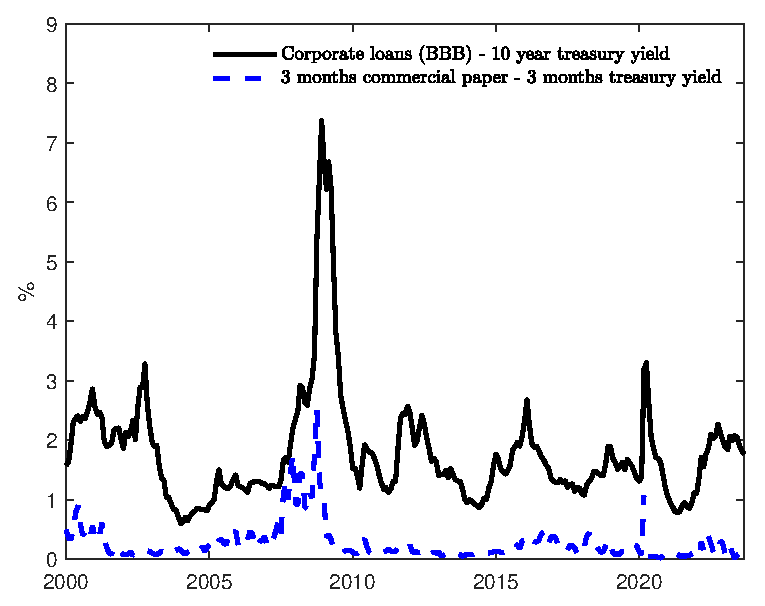
\includegraphics[height=0.80\textheight, keepaspectratio]{Figures/Figure21.eps}
    \end{column}

    % --- Text Column ---
    \begin{column}{0.35\textwidth}
        \scriptsize
        \begin{itemize}
            \item The figure illustrates the dramatic surge in credit spreads during both the 2008 crisis and the COVID-19 pandemic.
            \vspace{1em}
            \item It also demonstrates the central bank's ability to compress spreads and restore market functioning.
        \end{itemize}
    \end{column}

\end{columns}
\end{frame}

% --- SLIDE 60: Preview of Safe Assets ---
\begin{frame}{Looking Ahead: The Safe Asset Shortage}
\small

\textbf{The Liquidity Crunch Scenario}
\vspace{0.3em}
\begin{itemize}
    \item Chapter 11 will explore a scenario where the economy faces a critical shortage of "safe assets"—debts that serve as collateral or reliable stores of value.
\vspace{0.3em}
    \item The 2008 crisis revealed that private "money-like" securities (e.g., within the shadow banking system) lose their liquidity services exactly when needed most.
\vspace{0.3em}
\item The central bank  can counter the shortage of "safe assets" during a liquidity crisis by expanding reserves. 
\end{itemize}

\end{frame}

% ===================== SECTION: CONCLUSION =====================
\section{Conclusion}
% --- SLIDE 59: Summary I: Policy Tools ---
\begin{frame}{Main Takeaways: Concepts and Tools}
\small

\textbf{The liquidity trap}
\begin{itemize}
    \item Occurs when negative demand shocks interact with price rigidity and the ZLB.
    \item The result is a persistent shortfall in aggregate demand that cannot be cured by relying only on standard interest-rate cuts.
\end{itemize}

\vspace{0.2cm}

\textbf{Helicopter money}
\begin{itemize}
    \item Fiscal transfers financed by a permanent expansion of monetary liabilities.
    \item \textbf{Mechanism:} Raises long-run price expectations and stimulates consumption via the wealth effect, provided the liability increase is not offset by future taxes.
\end{itemize}

\vspace{0.2cm}

\textbf{Unconventional monetary policy (QE)}
\begin{itemize}
    \item Pure asset swaps are neutral in a frictionless model.
    \item To be effective, QE must induce a wealth transfer to the private sector—implying that the central bank or the Treasury absorbs risk and losses.
\end{itemize}
\end{frame}

\begin{frame}{Main Takeaways: Implementation Strategy}
\small

\textbf{Forward guidance}
\begin{itemize}
    \item Promises to keep rates at zero \emph{beyond} the duration of the shock.
    \item \textbf{History dependence:} allowing inflation to temporarily overshoot (“catch up”) lowers real interest rates and mitigates the recession.
    \item This approach allows the price level to reconnect with its trend in the long run.
\end{itemize}

\vspace{0.2cm}

\textbf{Managing reserves}
\begin{itemize}
    \item When reserves relax banking constraints, they should be increased aggressively during the trap and withdrawn gradually at liftoff.
    \item Fiscal policy (taxes) must adjust in a way that complements the liquidity policy.
\end{itemize}

\vspace{0.2cm}

\textbf{Financial stability}
\begin{itemize}
    \item The central bank acts as the buyer of last resort during systemic crises.
    \item Targeted credit‑easing operations prevent fire sales and stabilize spreads, complementing aggregate‑demand management.
\end{itemize}

\end{frame}

%% =====================================================
% =====================================================
\appendix
%% =====================================================
\section{Appendix}
% =====================================================

% --- SLIDE 10: Dynamics of central bank  Net Worth ---
\begin{frame}[label=Net]{Dynamics of central bank  Net Worth}
\small

\begin{itemize}
    \item For the constant price level $P^*$ to constitute an equilibrium, central bank  net worth must remain time-invariant. We analyze the evolution of net worth:
\end{itemize}
\textbf{Law of Motion}
    \begin{equation*}
        N_{t}^{C} = N_{t-1}^{C} + \Psi _{t}^{C} - T_{t}^{C} \label{NA_base}
    \end{equation*}
    \begin{itemize}
    \item Using the definition of net worth \eqref{DefNW}, profits represent the sum of the risk-free return on net assets and the risk premium earned on the bond portfolio:
    \begin{equation}
        \Psi _{t}^{C} = \underbrace{i_{t-1}(N_{t-1}^{C}+M_{t-1})}_{\text{Risk-free return}} + \underbrace{(i_{t}^{L}-i_{t-1})Q_{t-1}^{L}\tilde{B}_{L,t-1}^{C}}_{\text{Excess return on Long-Term Bonds}} \label{ProfitsCB}
    \end{equation}
    \item Substituting \eqref{ProfitsCB} into the law of motion:
    \begin{equation}
        N_{t}^{C} = (1+i_{t-1})N_{t-1}^{C} + i_{t-1}M_{t-1} + (i_{t}^{L}-i_{t-1})Q_{t-1}^{L}\tilde{B}_{L,t-1}^{C} - T_{t}^{C} \label{NA}
    \end{equation}
\end{itemize}
\end{frame}
% --- SLIDE 11: Proof of Net Worth Stability ---
\begin{frame}{Proof of Net Worth Stability}
\small
\begin{itemize}
    \item Substituting the transfer rule \eqref{Transfer} into \eqref{NA}.
    \item The variable components (profits/losses) cancel out, yielding:
    \begin{equation*}
        N_{t}^{C}=(1+i_{t-1})N_{t-1}^{C}-(1-\beta )P_{t}\tau ^{C}
    \end{equation*}
or
    \begin{equation*}
        N_{t}^{C}=N_{t-1}^{C}+P_{t}\left[\underbrace{i_{t-1}\frac{N_{t-1}^{C}}{P_{t}}-(1-\beta)\tau ^{C}}_{= \ 0} \right]
    \end{equation*}

\end{itemize}

\vspace{0.2cm}

\textbf{Conclusion}
\begin{itemize}
    \item From the equilibrium condition \eqref{CruxX} and since $i_{t-1} = \frac{1}{\beta}-1$, the term in brackets is identically zero, \textbf{net worth is constant} at the initial level: $N_{t}^{C}=N_{t-1}^{C} = N_{t_{0}-1}^{C}$.
\end{itemize}
\vspace{0.2cm}
\begin{center}
\hyperlink{Equilibrium}{\beamerbutton{Back to Equilibrium Price Level Stability}}
\end{center}
\end{frame}
\section{Bibliography}
\begin{frame}[allowframebreaks]{References}
    \printbibliography % 'heading=none' prevents double titles
\end{frame}

\end{document}
